\documentclass[
	% -- opções da classe memoir --
	12pt,				% tamanho da fonte
	openright,			% capítulos começam em pág ímpar (insere página vazia caso preciso)
	oneside,			% para impressão em verso e anverso. Oposto a oneside
	a4paper,			% tamanho do papel. 
	% -- opções da classe abntex2 --
	%chapter=TITLE,		% títulos de capítulos convertidos em letras maiúsculas
	%section=TITLE,		% títulos de seções convertidos em letras maiúsculas
	%subsection=TITLE,	% títulos de subseções convertidos em letras maiúsculas
	%subsubsection=TITLE,% títulos de subsubseções convertidos em letras maiúsculas
	% -- opções do pacote babel --
	english,			% idioma adicional para hifenização
	brazil				% o último idioma é o principal do documento
]{abntex2}

% ------------------------------------------------------
% Pacotes básicos 

\usepackage{unitins}
\usepackage{lmodern}			% Suporte tipografico completo
\renewcommand{\familydefault}{\sfdefault} % Define Arial (Sans-Serif) como fonte padrao do documento
\usepackage[T1]{fontenc}		% Selecao de codigos de fonte.
\usepackage[utf8]{inputenc}		% Codificacao do documento (conversão automática dos acentos)
\usepackage{lastpage}			% Usado pela Ficha catalográfica
\usepackage{indentfirst}		% Indenta o primeiro parágrafo de cada seção.
\usepackage[table,xcdraw]{xcolor} % Controle avançado de cores (substitui 'color' e integra tabelas)
\definecolor{lightgray}{gray}{0.9}

\usepackage{graphicx}			% Inclusão de gráficos
\usepackage{subcaption} 		% Subfiguras moderno (substitui subfig obsoleto)
\usepackage{microtype} 			% para melhorias de justificação
\usepackage{soul}
\usepackage{amssymb}
\usepackage{amsmath}
\usepackage{spreadtab}
\usepackage{multirow}
\usepackage{amsthm}
\usepackage{url}
\usepackage{listings}

\lstset{
	basicstyle=\ttfamily\footnotesize,
	breaklines=true,
	breakatwhitespace=false,
	columns=flexible,
	frame=single,
	numbers=left,
	numberstyle=\tiny,
	xleftmargin=1.5em,
	framexleftmargin=1em,
	showstringspaces=false,
	tabsize=2
}

% ------------------------------------------------------

\usepackage{hyperref}

% -----------------------------------------------
% Pacotes de citações

\usepackage[alf,abnt-etal-list=2,abnt-repeated-author-omit=yes]{abntex2cite}	% Citações padrão ABNT
\graphicspath{{imagens/}}           % Adicionar imagens

% --------------------------------------------

% ----------------------------------
%INCLUDE PDF 
\usepackage{pdfpages}
% ----------------------------------

% ----------------------------------------
% LONG TABLE - TABELA LONGA 

%\usepackage[margin=1in]{geometry}
\usepackage{longtable,tabularx,ltxtable}

\usepackage{threeparttablex} % for "ThreePartTable" environment
\usepackage{pgfplotstable}
\pgfplotsset{compat=1.18}
\usepackage{filecontents}
\usepackage{makecell}
\usepackage{booktabs}
\usepackage{float}

\citeoption{abnt-etal-cite=2}
% ---------------------------------------

\usepackage[running]{lineno}

% Dados do trabalho
\titulo{CONTROLE DE ACESSO IOT NA GESTÃO IMOBILIÁRIA VIA DSR}
\autor{ALÊKSON CASTRO DE SOUZA}
\local{Palmas}
\data{2026}
\orientador{Profa. Me. Tamirys Virgulino}
\instituicao{
Universidade Estadual do Tocantins\\
Curso de Sistemas de Informação
}

\tipotrabalho{Trabalho de Conclusão de Curso}

\preambulo{Trabalho de Conclusão de Curso apresentado ao Curso de Sistemas de Informação da Universidade Estadual do Tocantins como requisito parcial para obtenção do título de Bacharel.}


% ----
% Início do documento
% ----
\begin{document}

\imprimircapa
\imprimirfolhaderosto
\imprimirfichacatalografica
\imprimirfolhadeaprovacao

% Retira espaço extra obsoleto entre as frases.
\frenchspacing

% ----------------------------------------------------------
% ELEMENTOS PRÉ-TEXTUAIS
% ----------------------------------------------------------
% \pretextual
% ----------------------------------------------------------

\begin{resumo}
\SingleSpacing
\noindent
O modelo operacional de imobiliárias que gerenciam múltiplos corretores parceiros enfrenta um gargalo crítico no controle de acesso físico a propriedades dispersas. O compartilhamento tradicional de chaves metálicas e senhas de cofres mecânicos carece de rastreabilidade e apresenta riscos severos à segurança patrimonial. Embora fechaduras inteligentes conectadas mitiguem a distribuição de chaves, soluções vigentes pressupõem conectividade contínua à internet, inviabilizando sua aplicação no cenário mais frequente do setor: imóveis desocupados sem plano ativo de banda larga. Este trabalho propõe e avalia, sob a metodologia Design Science Research (DSR), um artefato de controle de acesso inteligente baseado em Internet das Coisas (IoT), validado em ambiente simulado, capaz de gerenciar com segurança o acesso temporário de múltiplos parceiros a imóveis desprovidos de conexão de rede. A solução integra controle de acesso baseado em atributos (ABAC contextual) a tokens criptográficos assinados digitalmente com o algoritmo de curva elíptica Ed25519, transmitidos via QR Code e verificados localmente pelo microcontrolador da fechadura em milissegundos, com sincronização assíncrona de auditoria via protocolo MQTT. A avaliação do artefato é estruturada por meio de simulação virtual em nós microcontrolados e testes automatizados de integração, estabelecendo métricas de latência temporal, ocupação de memória e eficácia de contenção lógica, com o intuito de fundamentar uma alternativa arquitetural de baixo custo e auditável no setor imobiliário.

\vspace{\onelineskip}
\noindent
\textbf{Palavras-chave}: Internet das Coisas (IoT). Controle de Acesso. Gestão Imobiliária. Criptografia Ed25519. Design Science Research.
\end{resumo}

\begin{resumo}[Abstract]
\SingleSpacing
\noindent
The operational model of real estate agencies managing multiple partner brokers faces a critical bottleneck in physical access control to dispersed properties. Traditional sharing of physical keys and lockbox passcodes lacks traceability and poses severe security risks. Although connected smart locks mitigate key handover logistics, current IoT solutions rely on continuous internet connectivity, failing in the sector's most common scenario: vacant properties without active broadband connections. This work proposes and evaluates, following the Design Science Research (DSR) methodology, an Internet of Things (IoT) intelligent access control artifact, validated in a simulated environment, capable of securely managing temporary access for multiple partners to offline properties. The solution couples Attribute-Based Access Control (contextual ABAC) with cryptographic tokens digitally signed via the Ed25519 elliptic curve algorithm, delivered through QR Codes and verified locally by the microcontrolled lock within milliseconds, alongside asynchronous audit synchronization via the MQTT protocol. The artifact evaluation is structured through virtual microcontroller simulation and automated integration tests, establishing performance metrics for latency, memory footprint, and logical containment efficacy, aiming to support an auditable and cost-effective architectural alternative tailored for real estate operations.

\vspace{\onelineskip}
\noindent
\textbf{Keywords}: Internet of Things (IoT). Access Control. Real Estate Management. Ed25519 Cryptography. Design Science Research.
\end{resumo}
\begin{siglas}
  \SingleSpacing
  \setlength{\itemsep}{0.1em}
  \item[ABAC] \textit{Attribute-Based Access Control} (Controle de Acesso Baseado em Atributos)
  \item[AES] \textit{Advanced Encryption Standard} (Padrão de Criptografia Avançada)
  \item[API] \textit{Application Programming Interface} (Interface de Programação de Aplicação)
  \item[ARM] \textit{Advanced RISC Machine} (Arquitetura de Processadores Embarcados)
  \item[BC-SNOA] \textit{Blockchain-based Secure and Non-interactive Offline Authentication}
  \item[BLE] \textit{Bluetooth Low Energy} (Bluetooth de Baixa Energia)
  \item[DSR] \textit{Design Science Research} (Metodologia de Pesquisa do Artefato)
  \item[ECC] \textit{Elliptic Curve Cryptography} (Criptografia de Curva Elíptica)
  \item[ECDSA] \textit{Elliptic Curve Digital Signature Algorithm}
  \item[Ed25519] \textit{Edwards-curve Digital Signature Algorithm 25519}
  \item[ESP32] Microcontrolador de Baixo Custo com Wi-Fi e Bluetooth Integrados
  \item[HABAC] \textit{Hierarchical Attribute-Based Access Control}
  \item[HMAC] \textit{Hash-based Message Authentication Code}
  \item[HTTP] \textit{Hypertext Transfer Protocol}
  \item[IoT] \textit{Internet of Things} (Internet das Coisas)
  \item[JSON] \textit{JavaScript Object Notation} (Formato de Carga Útil do Token)
  \item[MQTT] \textit{Message Queuing Telemetry Transport} (Protocolo de Mensageria Leve)
  \item[OTMP-P2L] \textit{One-Time Multi-Party Proof to Lock}
  \item[OTP] \textit{One-Time Password} (Senha de Uso Único)
  \item[PoW] \textit{Proof of Work} (Prova de Trabalho Criptográfica)
  \item[QR Code] \textit{Quick Response Code} (Código Bidimensional de Transporte do Token)
  \item[RBAC] \textit{Role-Based Access Control} (Controle de Acesso Baseado em Papéis)
  \item[SHA] \textit{Secure Hash Algorithm} (Função Hash Criptográfica)
  \item[TLS] \textit{Transport Layer Security} (Segurança da Camada de Transporte)
  \item[TTL] \textit{Time-To-Live} (Tempo de Vida Útil do Token)
  \item[Wi-Fi] \textit{Wireless Fidelity} (Rede Local sem Fio)
  \item[zk-SNARK] \textit{Zero-Knowledge Succinct Non-Interactive Argument of Knowledge}
\end{siglas}


\pdfbookmark[0]{\contentsname}{toc}
\tableofcontents*

\textual

% !TeX root = main.tex
\chapter{Introdução}
\label{cap:introducao}

% ============================================================
\section{Contextualização}
\label{sec:contextualizacao}
% ============================================================

O mercado imobiliário apoia-se em redes colaborativas de intermediação, nas quais administradoras gerenciam carteiras extensas de propriedades distribuídas geograficamente. Para viabilizar a comercialização e a locação desse patrimônio, as empresas dependem da atuação de dezenas de corretores autônomos e parceiros externos. Essa atividade impõe uma dinâmica operacional ágil e imprevista: visitas a imóveis costumam ser solicitadas por clientes em janelas de tempo reduzidas, com frequência fora do horário comercial, como no início da noite, intervalos de almoço ou finais de semana. Paralelamente às visitas comerciais, o ecossistema demanda acesso frequente para vistorias técnicas, serviços de limpeza, reparos de manutenção e registros fotográficos para divulgação em plataformas digitais.

Apesar da modernização dos sistemas de gestão e dos portais de anúncio, o controle de acesso físico às propriedades permanece dependente de métodos convencionais, centralizado no uso de chaves metálicas. Na prática, quando um corretor parceiro agenda um atendimento, precisa deslocar-se previamente até a sede da imobiliária para retirar o molho de chaves da unidade, assinar fichas de protocolo em papel, dirigir-se ao imóvel para a demonstração e, em seguida, retornar à sede para restituir o chaveiro. Esse procedimento gera atrito logístico constante: consome tempo excessivo em deslocamentos no trânsito, eleva despesas com combustível e frequentemente inviabiliza visitas quando a imobiliária encontra-se fechada, gerando perda de oportunidades comerciais.

Para contornar essa lentidão operacional, o mercado recorre a soluções de contingência frágeis, como deixar cópias com porteiros de condomínios sob guarda de terceiros ou instalar cofres mecânicos com segredo numérico (\textit{lockboxes}) presos a portões externos. Chaves físicas podem ser duplicadas em chaveiros comuns em poucos minutos sem qualquer registro formal \cite{camargosilvablockchain2023}. Já os cofres mecânicos utilizam senhas estáticas de quatro dígitos compartilhadas informalmente por aplicativos de mensagens instantâneas entre dezenas de profissionais, combinações que raramente são alteradas e mantêm o acesso aberto a corretores desvinculados por meses \cite{satanasaowapak2021}. O principal agravante desse cenário reside na total ausência de auditoria: caso ocorram avarias, torneiras abertas ou furtos de fiação, a administração não dispõe de meios para apurar quem acessou a unidade, em qual data e quanto tempo permaneceu no local.

A alternativa intuitiva seria a adoção de fechaduras inteligentes conectadas ao ecossistema de Internet das Coisas (\textit{Internet of Things} -- IoT). Entretanto, as opções comerciais vigentes foram projetadas para residências habitadas, operando sob a premissa de conexão ininterrupta a redes locais sem fio (Wi-Fi) vinculadas à nuvem \cite{vardakis2024}. Esse modelo colide com a realidade do setor: imóveis desocupados ofertados para venda ou locação encontram-se desprovidos de planos de banda larga fixa, visto que proprietários e administradores evitam assumir custos mensais de conexão durante o período de vacância. Sem infraestrutura de rede local no imóvel, os dispositivos convencionais tornam-se inoperantes ou recuam para o uso das mesmas chaves físicas, neutralizando os benefícios da automação.

Diante do dilema entre a necessidade de delegação ágil e a inexistência de conectividade no local, este trabalho desenvolve uma resposta arquitetural ao problema. A abordagem transfere a camada de conectividade para o único elemento provido de internet no instante da visita: o smartphone do corretor, que dispõe de conexão móvel celular (4G/5G). A fechadura embarcada opera de forma estritamente offline, utilizando criptografia de curvas elípticas (Ed25519) e avaliação dinâmica de políticas por atributos (ABAC contextual). O corretor requisita a permissão à nuvem, recebe o token assinado e o apresenta localmente via leitura óptica de QR Code; o microcontrolador valida a credencial matematicamente e aciona o destravamento, permitindo a sincronização assíncrona dos registros de auditoria via protocolo MQTT. A pesquisa é conduzida sob a metodologia \textit{Design Science Research} (DSR), orientando a concepção teórica, a implementação em bancada simulada e a avaliação experimental do artefato.

% ============================================================
\section{Problema de Pesquisa}
\label{sec:problema}
% ============================================================

O problema que orienta esta pesquisa desdobra-se em duas dimensões complementares: a operacional, decorrente da ausência de mecanismos centralizados e auditáveis para gerenciar o acesso temporário de parceiros; e a técnica, decorrente da exigência de conexão de rede nas soluções IoT convencionais, inoperantes em imóveis desocupados.

Diante desse cenário, define-se a seguinte pergunta de pesquisa:

\begin{quote}
\textit{Como projetar e avaliar uma arquitetura de controle de acesso inteligente baseada em IoT capaz de gerenciar, de forma segura, rastreável e orientada a atributos (ABAC), o acesso temporário de múltiplos corretores parceiros a imóveis desocupados desprovidos de conexão à internet?}
\end{quote}

% ============================================================
\section{Objetivo Geral}
\label{sec:objetivo-geral}
% ============================================================

Projetar e avaliar, por meio da metodologia \textit{Design Science Research} (DSR), um artefato IoT de controle de acesso que permita a imobiliárias gerenciar com segurança e rastreabilidade o acesso de corretores parceiros a imóveis offline, utilizando tokens assinados com o algoritmo Ed25519, validados em ambiente simulado.

% ============================================================
\section{Objetivos Específicos}
\label{sec:objetivos-especificos}
% ============================================================

\begin{enumerate}
    \item \textbf{Mapear o estado da arte} em autenticação offline, mensageria leve com MQTT (\textit{Message Queuing Telemetry Transport}) e criptografia de curva elíptica (ECC -- \textit{Elliptic Curve Cryptography}), de modo a fundamentar as decisões arquiteturais da proposta.
    \item \textbf{Modelar a arquitetura} do sistema em camadas, integrando controle de acesso baseado em atributos (ABAC contextual -- \textit{Attribute-Based Access Control}) a tokens Ed25519 verificáveis offline.
    \item \textbf{Implementar o protótipo simulado} cobrindo os cenários de acesso concedido, negado por violação de atributo e revogado.
    \item \textbf{Avaliar o protótipo} quanto à latência de verificação offline da assinatura Ed25519 no microcontrolador e à latência de comunicação MQTT na fase de emissão do token, além da eficácia na contenção de acessos indevidos.
\end{enumerate}

% ============================================================
\section{Justificativa}
\label{sec:justificativa}
% ============================================================

Os problemas mapeados na contextualização não são independentes: a falha operacional, o risco de segurança e a limitação tecnológica se reforçam mutuamente, e nenhuma solução disponível os endereça de forma integrada. É nessa interseção que o presente trabalho se posiciona, com justificativa distribuída em três planos:

\textbf{Plano prático.} A substituição de chaves físicas e senhas estáticas de \textit{lockboxes} elimina riscos de cópia não autorizada \cite{satanasaowapak2021} e reduz a dependência de plataformas proprietárias sujeitas a vazamento de credenciais \cite{camargosilvablockchain2023}, assegurando à imobiliária controle e auditoria confiáveis.

\textbf{Plano técnico.} Demonstra-se viável executar verificação criptográfica assimétrica por curvas elípticas (ECC) de maneira estritamente offline em microcontroladores de baixo custo, com tempo de resposta na ordem de milissegundos \cite{hanblockchainoffline2018,hanotmpp2l2020}.

\textbf{Plano acadêmico.} O estudo preenche a lacuna de integrar autenticação offline, políticas baseadas em atributos (ABAC contextual) e sincronização assíncrona de auditoria sob uma arquitetura voltada ao setor imobiliário.

% ============================================================
\section{Estrutura do Trabalho}
\label{sec:estrutura}
% ============================================================

O trabalho organiza-se em cinco capítulos: o Capítulo \ref{cap:fundamentacao} apresenta a fundamentação teórica e os trabalhos correlatos; o Capítulo \ref{cap:metodologia} descreve o método DSR adotado; o Capítulo \ref{cap:resultados} apresenta a arquitetura, o protótipo simulado e a avaliação experimental; e o Capítulo \ref{cap:conclusao} sintetiza as contribuições e propõe trabalhos futuros.

% !TeX root = main.tex
\chapter{Fundamentação Teórica}
\label{cap:fundamentacao}

Este capítulo apresenta a base teórica e tecnológica que sustenta a concepção e a modelagem do artefato proposto neste trabalho. A discussão está estruturada em quatro eixos temáticos: (i) Internet das Coisas (IoT), sua arquitetura em camadas e protocolos de mensageria leve; (ii) modelos de controle de acesso e autorização dinâmica em ambientes computacionais restritos, incluindo a criptografia assimétrica para validação offline em dispositivos de borda; (iii) fechaduras inteligentes, acompanhadas de análise comparativa do estado da arte, com ênfase em esquemas de autenticação sem conectividade de rede; e (iv) segurança, rastreabilidade e trilhas de auditoria em ecossistemas IoT.

% ============================================================
\section{Internet das Coisas (IoT): Conceitos e Arquitetura}
\label{sec:iot}
% ============================================================

\subsection{Definição e Desafios em Dispositivos Conectados}
\label{subsec:iot-definicao}

A Internet das Coisas (\textit{Internet of Things} -- IoT) consiste na interconexão digital de objetos físicos à infraestrutura de rede, permitindo que sensores, atuadores e microcontroladores realizem a coleta, o processamento e a troca autônoma de dados sem intervenção humana contínua \cite{vardakis2024}.

Entretanto, \citeonline{vardakis2024} e \citeonline{ssaac2022} ressaltam que o avanço da IoT expõe desafios críticos de segurança decorrentes da heterogeneidade e da severa restrição computacional dos nós de borda. Ao contrário de servidores de aplicação ou estações de trabalho, dispositivos embarcados em extremidades de rede operam com processadores de baixo custo, memória volátil reduzida e capacidade energética limitada. Tal restrição inviabiliza a execução local de pilhas criptográficas complexas ou algoritmos pesados de avaliação de políticas de segurança \cite{surveysmarthomeauth2021}. 

Diante desse cenário, torna-se imperativo projetar arquiteturas computacionais que dissociem a tarefa de decisão de acesso da tarefa de atuação física. Essa diretriz fundamenta diretamente o desenvolvimento do presente trabalho, no qual o dispositivo de acionamento da trava no imóvel atua exclusivamente na execução de ordens validadas previamente por uma infraestrutura centralizada.

\subsection{Arquitetura em Camadas e Gateways de Borda}
\label{subsec:iot-arquitetura}

A literatura científica adota predominantemente a representação de sistemas IoT organizada em quatro camadas hierárquicas, estruturando o fluxo de dados desde a captura física até a interação com o usuário final \cite{vardakis2024}:

\begin{enumerate}
    \item \textbf{Camada Física e de Percepção:} Abrange o hardware embarcado, atuadores mecânicos (fechaduras elétricas ou solenóides), sensores de presença e leitores de entrada de credenciais (interfaces de leitura de QR Code, biometria ou teclados).
    \item \textbf{Camada de Rede:} Fornece a infraestrutura de transmissão de dados via enlaces locais (Wi-Fi, Bluetooth) ou remotos, conectando dispositivos locais aos servidores de controle por meio de protocolos de transporte e aplicação dedicados.
    \item \textbf{Camada de Middleware e Processamento:} Responsável pelo processamento lógico, aplicação de políticas de autorização, gerenciamento de regras temporais e persistência de dados.
    \item \textbf{Camada de Aplicação:} Engloba os painéis administrativos web e aplicativos móveis voltados aos administradores imobiliários e aos corretores autorizados.
\end{enumerate}

Para mitigar a vulnerabilidade decorrente da exposição direta de microcontroladores à internet pública, \citeonline{vardakis2024} e \citeonline{ameer2022} preconizam a inserção de um \textit{gateway} local ou de borda (\textit{edge gateway}). O gateway centraliza a comunicação local, atua como intermediário na validação criptográfica e isola os dispositivos físicos de varreduras externas de rede. 


\subsection{Protocolo de Mensageria Leve: MQTT}
\label{subsec:mqtt}

O MQTT (\textit{Message Queuing Telemetry Transport}) é um protocolo de mensageria assíncrona baseado no padrão de publicação e subscrição (\textit{publish/subscribe}), concebido especificamente para redes com largura de banda limitada e dispositivos com recursos restritos \cite{ameer2022}. No modelo MQTT, clientes publicam mensagens associadas a tópicos específicos em um intermediário central (\textit{broker}), o qual roteia os dados unicamente para os clientes previamente inscritos nesses mesmos canais de interesse.

Em sistemas de segurança física, o MQTT viabiliza o envio imediato e bidirecional de comandos e telemetrias com sobrecarga (\textit{overhead}) de cabeçalho substancialmente inferior àquela gerada pelo protocolo HTTP tradicional \cite{shauto2024}. \citeonline{ameer2022} demonstraram que a aplicação de MQTT combinada à criptografia de transporte via TLS (\textit{Transport Layer Security}) oferece canais resilientes e com tempos de propagação de mensagens da ordem de milissegundos, impedindo a interceptação passiva e a adulteração de comandos de acionamento. Ademais, \citeonline{simperf2024} validam experimentalmente que o MQTT associado a microcontroladores como o ESP32 mantém estabilidade de latência em cenários simulados de controle de tráfego.

Essa eficiência operacional orienta a escolha do MQTT no artefato deste estudo, viabilizando o despacho em tempo real do evento de abertura para a fechadura imediatamente após a validação da permissão do corretor pelo servidor.

% ============================================================
\section{Controle de Acesso em Ambientes IoT}
\label{sec:controle-acesso}
% ============================================================

\subsection{Controle de Acesso Baseado em Papéis (RBAC) e Suas Limitações}
\label{subsec:rbac}

O modelo de Controle de Acesso Baseado em Papéis (\textit{Role-Based Access Control} -- RBAC) fundamenta-se na concessão de privilégios a determinados papéis organizacionais (\textit{roles}), atribuindo posteriormente os usuários a essas categorias pré-definidas \cite{ameer2022}. Trata-se do padrão amplamente implementado em sistemas de informação corporativos tradicionais devido à simplicidade administrativa inicial que oferece.

Contudo, investigações recentes apontam que o RBAC apresenta rigidez excessiva quando transposto para ambientes ubíquos e IoT dinâmicos \cite{ameer2022, surveysmarthomeauth2021}. Em um ecossistema imobiliário, por exemplo, a atribuição estática do papel ``Corretor'' revela-se insuficiente para a segurança da operação: conceder acesso ilimitado com base apenas na função profissional impediria restringir o acesso a um imóvel específico, a uma faixa de horário comercial determinada ou a uma data de agendamento confirmada. Para reproduzir tais restrições no RBAC, o administrador seria obrigado a multiplicar papéis de forma insustentável (\textit{role explosion}) \cite{ameer2022}.

Portanto, evidencia-se a necessidade de adotar modelos mais expressivos, capazes de fundamentar decisões de autorização em dados contextuais em vez de relações binárias entre usuários e funções organizacionais.

\subsection{Controle de Acesso Baseado em Atributos (ABAC) e o Modelo \texorpdfstring{HABAC$\alpha$}{HABAC-Alpha}}
\label{subsec:abac}

O Controle de Acesso Baseado em Atributos (\textit{Attribute-Based Access Control} -- ABAC) supera as limitações do RBAC ao computar permissões a partir da avaliação dinâmica de atributos pertencentes a quatro categorias: sujeito (identidade do usuário, certificação do corretor), recurso (identificador do imóvel, estado da fechadura), ação pretendida (destravar, auditar) e ambiente (data, hora, geolocalização ou duração da visita) \cite{ameer2022, continuousauth2022}.

A flexibilidade do ABAC foi aprimorada por \citeonline{ameer2022} na formulação do modelo HABAC$\alpha$ (\textit{Home Attribute-Based Access Control}), voltado ao ecossistema de residências inteligentes. O HABAC$\alpha$ formaliza políticas de autorização sensíveis ao contexto que consideram a hierarquia espacial do imóvel e condicionantes temporais estritas. Sob o HABAC$\alpha$, a autorização deixa de ser uma permissão perpétua e torna-se um evento transitório, revogado no instante em que qualquer condição contextual (como o término do horário estipulado) for violada \cite{ameer2022}.

Essa formulação conceitual é diretamente transposta para a arquitetura desta pesquisa: o corretor parceiro apenas obtém acesso ao imóvel se preencher concomitantemente o vínculo ativo com a imobiliária, o agendamento prévio cadastrado e a janela cronológica precisa da visita.

\subsection{Autenticação Temporária por Tokens Efêmeros}
\label{subsec:tokens}

Para que as políticas avaliadas pelo motor ABAC sejam executadas com agilidade na ponta sem sobrecarregar a fechadura, adota-se o paradigma de autenticação temporária desacoplada mediante tokens efêmeros \cite{satanasaowapak2021}. Sob essa abordagem, a infraestrutura central de autorização gera um código criptográfico temporizado dotado de tempo de vida útil reduzido (\textit{Time-To-Live} -- TTL), entregue digitalmente ao dispositivo do solicitante.

\citeonline{satanasaowapak2021} propuseram um sistema de fechadura inteligente baseado em tokens descartáveis e senhas temporárias (OTP), demonstrando que o uso de credenciais que expiram automaticamente anula o risco associado ao roubo, compartilhamento ou vazamento posterior de senhas estáticas. De modo complementar, \citeonline{ssaac2022} ressaltam que tokens efêmeros permitem delegar ao cliente a comprovação de sua legitimidade com baixíssima complexidade de checagem no dispositivo de atuação.

Assim, a geração de tokens dinâmicos no artefato deste TCC garante que a chave digital permaneça válida estritamente pelo intervalo necessário para a vistoria do imóvel, impedindo reutilizações indevidas por corretores ou terceiros após o término do evento.

\subsection{Criptografia Assimétrica e Verificação Offline em Dispositivos de Borda}
\label{subsec:criptografia-assimetrica}

A adoção de criptografia assimétrica baseada em curvas elípticas (ECC --- \textit{Elliptic Curve Cryptography}) representa uma solução computacionalmente viável para implementar autenticação robusta em microcontroladores restritos sem depender de conectividade de rede no momento do acesso \cite{hanblockchainoffline2018}. Ao contrário de protocolos simétricos que exigem o compartilhamento prévio de um segredo entre remetente e receptor, o modelo assimétrico separa claramente as responsabilidades: a chave privada, custodiada com exclusividade pelo servidor central, assina digitalmente o token de acesso durante a fase de agendamento online; a chave pública correspondente, gravada em memória não volátil do microcontrolador, executa apenas a verificação criptográfica dessa assinatura no momento do destravamento \cite{hanotmpp2l2020}.

Essa dissociação atende diretamente ao cenário de imóveis desocupados sem infraestrutura de rede local: o dispositivo de borda não precisa consultar qualquer servidor para validar a autenticidade e a vigência da credencial. O processo de verificação de uma assinatura ECC é uma operação matemática de custo computacional reduzido e tempo constante, executável em centenas de milissegundos mesmo em processadores de baixo consumo energético. \citeonline{hanotmpp2l2020} validaram experimentalmente essa premissa ao construir um protótipo de fechadura inteligente offline com validação completa em apenas 339 milissegundos em um microcontrolador ARM Cortex-A7, demonstrando que a arquitetura de verificação local alia rigor de segurança à agilidade operacional para o usuário final.

A curva Ed25519, variante de assinatura de alta performance derivada da Curve25519, destaca-se nesse contexto por oferecer chaves de apenas 32 bytes, assinaturas de 64 bytes e resistência comprovada a ataques de canal lateral, sendo implementada nativamente nas principais bibliotecas de criptografia embarcada \cite{hanblockchainoffline2018}. Esse conjunto de propriedades fundamenta a escolha do esquema de assinatura digital assimétrica como mecanismo central de autenticação offline no artefato proposto neste trabalho.

% ============================================================
\section{Fechaduras Inteligentes e Trabalhos Relacionados}
\label{sec:fechaduras}
% ============================================================

\subsection{Limitações dos Mecanismos Tradicionais de Acesso Físico}
\label{subsec:limitacoes-tradicionais}

Os mecanismos tradicionais de controle de acesso a imóveis dependem prioritariamente de chaves metálicas mecânicas ou de cartões magnéticos e códigos numéricos estáticos \cite{satanasaowapak2021, camargosilvablockchain2023}. No contexto operacional de imobiliárias que gerenciam dezenas ou centenas de propriedades distribuídas geograficamente, esse paradigma acarreta severas deficiências práticas.

Primeiramente, o manuseio de chaves físicas impõe sobrecarga logística, exigindo que corretores parceiros desloquem-se até a sede da empresa apenas para retirar e devolver os chaveiros, além de expor os proprietários ao risco de clonagem clandestina de lâminas metálicas sem qualquer vestígio \cite{satanasaowapak2021}. Em segundo lugar, senhas estáticas compartilhadas por mensagens informais tendem a ser repassadas entre corretores e prestadores de serviços, tornando impossível assegurar quem de fato acessou o recinto \cite{camargosilvablockchain2023}. Finalmente, tais métodos não produzem registros automatizados de entrada e saída, impedindo auditorias eficientes caso ocorram furtos ou danos aos imóveis.

O Quadro~\ref{quadro:comparativo-metodos} sintetiza as principais características e fragilidades desses métodos frente aos requisitos demandados pelo cenário investigado e pelo artefato proposto.

\begin{table}[htbp]
\centering
\footnotesize
\caption{Comparação entre métodos convencionais de controle de acesso e o artefato proposto.}
\label{quadro:comparativo-metodos}
\begin{tabularx}{\textwidth}{p{3.2cm}cccX}
\toprule
\textbf{Método} & \textbf{Rastreabilidade} & \textbf{Revogação} & \textbf{Modo Offline} & \textbf{Limitação Principal} \\
\midrule
Chave física metálica & Não & Não & Sim & Risco de cópia ou extravio não registrado \cite{camargosilvablockchain2023}. \\
Cofre mecânico com segredo (\textit{lockbox}) & Não & Não & Sim & Senhas estáticas repassadas informalmente entre dezenas de corretores. \\
Teclado numérico local (\textit{PIN pad}) & Não & Parcial & Sim & Vulnerável à observação de terceiros (\textit{shoulder surfing}) e ataques de força bruta \cite{shauto2024}. \\
Fechadura inteligente comercial (Wi-Fi) & Sim & Sim & Não & Depende de conexão fixa local com servidores do fabricante \cite{vardakis2024}. \\
\textbf{Artefato proposto (DSR)} & \textbf{Sim} & \textbf{Sim} & \textbf{Sim} & \textbf{Validação por chave pública e delegação por token com TTL.} \\
\bottomrule
\end{tabularx}
\fonte{Elaborado pelo autor (2026).}
\end{table}

\subsection{Sistemas de Fechaduras Baseados em IoT}
\label{subsec:fechaduras-iot}

A substituição de cilindros mecânicos por fechaduras inteligentes conectadas (\textit{smart locks}) transforma o ponto de acesso em um nó computacional autônomo. O acionamento da tranca passa a ser intermediado por sinais eletrônicos condicionados à verificação de credenciais digitais móveis, biometria facial ou leitura de códigos bidimensionais (QR Codes) \cite{satanasaowapak2021, yolov5smartlock2025}.

Diversos projetos acadêmicos e comerciais vêm aplicando essa transição. \citeonline{yolov5smartlock2025} utilizam visão computacional embarcada para identificação facial em fechaduras inteligentes residenciais. Contudo, conforme apontado por \citeonline{shauto2024}, abordagens dependentes exclusivamente de hardware biométrico local aumentam exponencialmente o custo unitário por porta, além de criarem barreiras de privacidade e exigirem o cadastramento facial prévio de todos os corretores parceiros em cada dispositivo instalado. Por sua vez, fechaduras comerciais dependentes de nuvens proprietárias expõem o administrador ao confinamento tecnológico (\textit{vendor lock-in}) e a custos contínuos de assinatura \cite{camargosilvablockchain2023}.

Nesse cenário, dois trabalhos acadêmicos se destacam pela abordagem pioneira de autenticação offline em fechaduras inteligentes. \citeonline{hanblockchainoffline2018} propuseram o BC-SNOA (\textit{Blockchain-based Succinct Non-interactive Offline Authentication}), um esquema que combina criptografia de curva elíptica (ECC --- Secp256k1), Prova de Trabalho (PoW) baseada em SHA-256 e provas de conhecimento zero (zk-SNARKs) para permitir que a fechadura valide o QR Code apresentado pelo usuário de forma completamente offline, sem consultar qualquer servidor ou nuvem no momento do destravamento. O token é gerado durante a fase de reserva online e encapsulado em um código QR entregue ao smartphone do usuário; na porta, a fechadura executa a verificação matemática local e aciona o mecanismo de abertura sem qualquer dependência de conectividade.

\citeonline{hanotmpp2l2020} avançaram sobre essa proposta com o esquema OTMP-P2L (\textit{One-Time Association Multitask Proofs for Peer to Local Authentication}), estruturado em torno de provas de conhecimento zero encadeadas baseadas em problemas NP: prova de período temporal (ECC homomórfico), prova de token legítimo (HMAC e assinatura ECC), prova de trabalho (PoW SHA-256) e verificação de pertencimento ao grupo por meio do acumulador unidirecional de Nyberg. Em testes físicos com microcontrolador ARM Cortex-A7 e leitor de QR Code, os autores alcançaram tempo de validação completa de apenas 339 milissegundos e tamanho de token de 593 bytes --- resultados que demonstram a plena viabilidade da abordagem em hardware restrito de baixo custo.


\subsection{Análise Comparativa do Estado da Arte}
\label{subsec:trabalhos-relacionados}

Para fundamentar as escolhas arquiteturais e demonstrar a lacuna tecnológica atendida por esta pesquisa, o Quadro \ref{quadro:trabalhos-relacionados} sintetiza a comparação crítica entre as principais soluções identificadas na literatura recente frente à proposta deste trabalho.

\begin{table}[htbp]
\centering
\footnotesize
\setlength{\tabcolsep}{4pt}
\renewcommand{\arraystretch}{0.95}
\caption{Comparação entre soluções da literatura e a arquitetura proposta.}
\label{quadro:trabalhos-relacionados}
\begin{tabular}{p{3.2cm}p{2.3cm}p{2.5cm}p{2.4cm}p{3.8cm}}
\toprule
\textbf{Trabalho / Autor} & \textbf{Mecanismo} & \textbf{Protocolo} & \textbf{Controle / Aut.} & \textbf{Lacuna Identificada} \\
\midrule
\citeonline{satanasaowapak2021} & OTP / Token Web & HTTP / Web Server & Estático temporizado & Dependência de servidor web local; sem suporte ABAC contextual. \\
\addlinespace
\citeonline{ameer2022} (HABAC$\alpha$) & Atributos / App & MQTT / TLS & ABAC formal hierárquico & Focado em residências unifamiliares; não aborda terceirização ou múltiplos parceiros. \\
\addlinespace
\citeonline{vardakis2024} & Gateway Smart Home & Não especificado & Baseado em papéis & Abordagem genérica de segurança; ausência de protótipo de acesso físico. \\
\addlinespace
\citeonline{camargosilvablockchain2023} & Smart Contracts / IoT & Blockchain & Descentralizado / P2P & Alta sobrecarga computacional e latência de mineração; inviável em cenários de baixo custo. \\
\addlinespace
\citeonline{shauto2024} & Biometria / Senha & Wi-Fi / Cloud & Autenticação local & Custo elevado por nó; vulnerável ao compartilhamento presencial de senhas. \\
\addlinespace
\citeonline{yolov5smartlock2025} & Visão (YOLOv5) & Rede local & Reconhecimento Facial & Alto consumo de processamento; exige pré-cadastro de faces para cada corretor. \\
\addlinespace
\citeonline{hanblockchainoffline2018} (BC-SNOA) & ECC + PoW + zk-SNARK + QR Code & Nenhum (offline) & Criptográfico offline & Contexto de reserva de salas corporativas; sem ABAC imobiliário; sem ESP32. \\
\addlinespace
\citeonline{hanotmpp2l2020} (OTMP-P2L) & ECC + PoW + HMAC + Acumulador Nyberg & Nenhum (offline) & Provas NP encadeadas & Prova de conceito em ARM; sem rastreabilidade de auditoria; sem contexto imobiliário. \\
\midrule
\textbf{Artefato Proposto} & \textbf{Token Ed25519 / ABAC} & \textbf{QR Code Offline} & \textbf{ABAC Contextual Offline} & \textbf{Baixo custo, validação 100\% offline sem Wi-Fi no imóvel, múltiplos parceiros e trilha completa de auditoria.} \\
\bottomrule
\end{tabular}
\fonte{Elaborado pelo autor (2026).}
\end{table}

A comparação evidenciada no Quadro \ref{quadro:trabalhos-relacionados} ratifica que, conquanto existam iniciativas sofisticadas baseadas em blockchain \cite{camargosilvablockchain2023} ou visão computacional \cite{yolov5smartlock2025}, persiste uma carência de arquiteturas enxutas que combinem baixo custo de implantação, autorização contextual dinâmica (ABAC) e auditoria transparente para ambientes corporativos com múltiplos atores externos.

% ============================================================
\section{Segurança, Rastreabilidade e Auditoria em Sistemas IoT}
\label{sec:seguranca}
% ============================================================

\subsection{Vetores de Ataque e Vulnerabilidades Comuns}
\label{subsec:ameacas}

No modelo proposto, três vetores de ataque são especialmente críticos: a interceptação do token em trânsito, a reutilização de um QR Code já utilizado e o uso indevido do smartphone do corretor como ponto de decisão de segurança \cite{shauto2024, surveysmarthomeauth2021}. A espionagem passiva (\textit{eavesdropping}), os ataques de repetição (\textit{replay attacks}) e a interceptação ativa (\textit{man-in-the-middle}) são os mecanismos concretos associados a esses vetores \cite{shauto2024}. A ausência de criptografia de transporte no MQTT permitiria que um invasor capturasse o comando de abertura e o replicasse para destrancar o imóvel em momento posterior.

Em cenários de validação offline, o risco de reutilização de tokens persiste mesmo sem acesso à rede: um atacante que capture o QR Code durante uma visita pode tentar apresentá-lo novamente após o encerramento da janela temporal autorizada. Para neutralizar essa ameaça, o artefato proposto associa a cada token um identificador único de uso único (\textit{nonce} --- campo \texttt{jti} do JWT), cujo registro é persistido em buffer circular na memória não volátil (NVS Flash) do microcontrolador, garantindo que nenhum token já processado seja aceito novamente, independentemente de sua validade criptográfica \cite{hanotmpp2l2020}.

Adicionalmente, \citeonline{zhoumaag2022} mapearam sistematicamente as vulnerabilidades introduzidas pelo paradigma \textit{Mobile-as-a-Gateway} (MaaG), no qual o smartphone do usuário atua não como simples transportador, mas como árbitro ativo das políticas de acesso. Os autores identificaram quatro classes críticas de falha --- perda semântica na tradução de permissões, responsabilidades assimétricas entre nuvem e dispositivo, inconsistência causal na sincronização e injeção de chaves ocultas locais --- que permitem a usuários temporários manter acesso indefinido ao dispositivo físico mesmo após revogação no servidor. Esse diagnóstico fundamenta uma decisão arquitetural central no presente trabalho: o smartphone do corretor atua exclusivamente como transportador passivo do token assinado, sem poder de decisão ou armazenamento de regras de acesso; toda a lógica de validação reside no microcontrolador.

No plano das credenciais, o emprego de senhas estáticas ou padrões PIN perpetua vulnerabilidades de força bruta e captura por engenharia social \cite{shauto2024}. Paralelamente, como advertem \citeonline{camargosilvablockchain2023}, a dependência irrestrita de serviços em nuvem proprietários de terceiros introduz o perigo de exfiltração não controlada de registros de acesso ou de indisponibilidade unilateral dos servidores remotos durante vistorias essenciais.

\subsection{Mecanismos de Proteção e Trilhas de Auditoria}
\label{subsec:mecanismos}

Para mitigar integralmente as fragilidades delineadas, a arquitetura do artefato adota uma estratégia de defesa em profundidade estruturada em quatro pilares técnicos complementares:

\begin{enumerate}
    \item \textbf{Criptografia de Transporte (TLS):} Blindagem criptográfica fim a fim de todos os pacotes MQTT trafegados entre os clientes, o broker e o microcontrolador, inviabilizando técnicas de leitura e injeção maliciosa de pacotes \cite{ameer2022, shauto2024}.
    \item \textbf{Descarte Temporal de Credenciais:} Configuração de expiração algorítmica estrita (TTL curto) associada a cada token gerado, eliminando os impactos de vazamento de credenciais pós-uso \cite{satanasaowapak2021}.
    \item \textbf{Isolamento em Gateway Local:} Centralização da tomada de decisão no gateway de borda, preservando a fechadura contra conexões diretas oriundas da internet pública \cite{vardakis2024, ameer2022}.
    \item \textbf{Trilha Auditável de Eventos (\textit{Audit Trail}):} Persistência sequencial imutável de todos os eventos de autorização, abrangendo concessões legítimas, recusas de tentativas fora do expediente e revogações forçadas de acesso \cite{shauto2024}.
\end{enumerate}

A consolidação de logs auditáveis atende com rigor à necessidade de transparência demandada pela governança imobiliária: a qualquer instante, a administração dispõe de comprovação cabal de qual corretor solicitou a entrada, o instante exato de liberação e o tempo decorrido até o trancamento, estabelecendo a responsabilização inequívoca pelo patrimônio administrado.

\bigskip
Dessa forma, o conjunto de conceitos, protocolos e modelos analíticos delineados neste capítulo fornece o embasamento teórico e a justificativa técnica necessários para a formalização metodológica e o desenvolvimento do protótipo simulado nos capítulos subsequentes.
% !TeX root = main.tex
\chapter{Metodologia de Pesquisa}
\label{cap:metodologia}

Este capítulo descreve os procedimentos metodológicos adotados para a concepção, o desenvolvimento e a avaliação experimental do artefato proposto. O trabalho apoia-se nas diretrizes da \textit{Design Science Research} (DSR), método voltado à resolução de problemas organizacionais mediante a criação e avaliação rigorosa de artefatos computacionais \cite{hevner2004,peffers2007}.

% ============================================================
\section{Caracterização Metodológica}
\label{sec:dsr-caracterizacao}
% ============================================================

\subsection{Design Science Research como Paradigma}
\label{subsec:dsr-paradigma}

A pesquisa em computação aplicada comporta abordagens explicativas e prescritivas. Enquanto as ciências comportamentais focam na observação de fenômenos, a DSR orienta-se pela produção de conhecimento por meio da construção e da validação empírica de artefatos --- constructos, modelos, métodos e instanciações \cite{hevner2004}. 

A gestão de visitas em imóveis desocupados apresenta gargalos operacionais e vulnerabilidades que decorrem de métodos manuais (chaves físicas e senhas estáticas) e da ausência de internet local nos imóveis. A resposta a essa demanda requer a especificação de modelos formais e a implementação de protótipos funcionais. A condução do estudo segue o modelo de processo de seis etapas estabelecido por \citeonline{peffers2007}, estruturado conforme o Quadro~\ref{quadro:mapeamento-dsr}.

\begin{table}[htbp]
\centering
\footnotesize
\caption{Mapeamento das etapas da Design Science Research no projeto.}
\label{quadro:mapeamento-dsr}
\begin{tabularx}{\textwidth}{c p{3.8cm} X p{3.0cm}}
\toprule
\textbf{Fase} & \textbf{Etapa \cite{peffers2007}} & \textbf{Atividade Realizada} & \textbf{Localização} \\
\midrule
1 & Identificação do Problema & Diagnóstico das falhas de segurança e logística em imóveis vagos sem conectividade. & Seção~\ref{sec:problema-contexto} e Cap.~\ref{cap:introducao} \\
\addlinespace
2 & Definição dos Objetivos & Definição dos requisitos de projeto, pilares arquiteturais e metas quantitativas. & Seção~\ref{subsec:pilares-artefato} e Seção~\ref{sec:metricas-avaliacao} \\
\addlinespace
3 & Projeto e Desenvolvimento & Concepção do modelo HABAC$\alpha$, esquema Ed25519, firmware ESP32 e API FastAPI. & Cap.~\ref{cap:resultados} \\
\addlinespace
4 & Demonstração & Execução do fluxo nominal, testes negativos de ataque e revogação em bancada virtual. & Seção~\ref{sec:cenarios-teste} e Cap.~\ref{cap:resultados} \\
\addlinespace
5 & Avaliação Experimental & Coleta de latência, memória e eficácia de bloqueio em 50 repetições com análise estatística. & Seção~\ref{sec:metricas-avaliacao} e Cap.~\ref{cap:resultados} \\
\addlinespace
6 & Comunicação & Redação acadêmica, sistematização de diagramas e discussão comparativa dos dados. & Monografia \\
\bottomrule
\end{tabularx}
\fonte{Elaborado pelo autor (2026).}
\end{table}

% ============================================================
\section{Contexto e Formalização do Problema}
\label{sec:problema-contexto}
% ============================================================

\subsection{Cenário de Gestão de Visitas e Análise dos Métodos Vigentes}
\label{subsec:cenario-imobiliario}

Imobiliárias administram carteiras distribuídas de unidades desocupadas cuja comercialização depende de corretores parceiros e prestadores de serviços. A operação caracteriza-se por três restrições: (i) ausência de conexão de rede local (Wi-Fi ou cabeada), visto que custos de banda larga não são mantidos na vacância; (ii) inexistência de fiscalização física no local; e (iii) elevada rotatividade de profissionais que necessitam de janelas de entrada temporárias e pontuais.

Conforme analisado no Quadro~\ref{quadro:comparativo-metodos} (Seção~\ref{subsec:limitacoes-tradicionais}), os métodos convencionais mostram-se inadequados: chaves metálicas causam atrito logístico e risco de cópias; cofres mecânicos empregam senhas estáticas compartilhadas sem rastreabilidade; e fechaduras comerciais conectadas dependem de Wi-Fi local ininterrupto, tornando-se inoperantes em imóveis desocupados.

\subsection{Questão de Pesquisa e Pilares do Artefato}
\label{subsec:questao-pesquisa}

A incapacidade dos mecanismos atuais de conciliar operação desconectada, controle contextual e auditoria orienta a questão de pesquisa:

\begin{quote}
\textit{Como projetar e avaliar uma arquitetura de controle de acesso inteligente baseada em IoT capaz de gerenciar, de forma segura, rastreável e orientada a atributos (ABAC), o acesso temporário de múltiplos corretores parceiros a imóveis desocupados desprovidos de conexão à internet?}
\end{quote}

\label{subsec:pilares-artefato}
Para orientar a construção do artefato, definiram-se quatro pilares técnicos:
\begin{enumerate}
    \item \textbf{Independência de rede local (\textit{Zero Local Infrastructure}):} Validação matemática de credenciais na borda sem consulta a servidores remotos e sem modems dedicados na fechadura.
    \item \textbf{Autenticidade e não-repúdio:} Delegação assinada por autoridade central e vinculada ao dispositivo móvel habilitado do corretor.
    \item \textbf{Autorização orientada a atributos (ABAC):} Liberação condicionada a atributos de sujeito, objeto, ação e ambiente avaliados em tempo de execução.
    \item \textbf{Auditoria assíncrona:} Registro inviolável de acessos e sincronização com a nuvem utilizando o smartphone do corretor como portador de dados (\textit{data mule}).
\end{enumerate}

% ============================================================
\section{Procedimentos e Instrumentos de Avaliação}
\label{sec:procedimentos-avaliacao}
% ============================================================

\subsection{Ambiente de Simulação Virtual}
\label{subsec:justificativa-wokwi}

A avaliação do artefato adota a simulação virtual no Wokwi Simulator \cite{simperf2024}. A opção justifica-se por três fatores: (i) reprodutibilidade científica integral dos ensaios de temporização em ambiente controlado; (ii) isolamento de variáveis espúrias mecânicas ou térmicas de protoboards na medição da computação criptográfica; e (iii) viabilidade experimental de testes de estresse sem degradação física de atuadores solenoide.

\subsection{Planejamento dos Cenários de Demonstração}
\label{sec:cenarios-teste}

A validação funcional divide-se em três cenários planejados:
\label{subsec:cenario-1}
\textbf{Cenário 1 (Fluxo nominal):} Avalia a solicitação de token por corretor cadastrado para imóvel liberado em horário comercial. Critério de sucesso: emissão do token, validação no microcontrolador em menos de 10~ms, acionamento do relé por 5 segundos e entrega do recibo de telemetria via MQTT sob QoS 1.

\label{subsec:cenario-2}
\textbf{Cenário 2 (Ensaios negativos e ataques):} Avalia a capacidade de rejeição local do firmware frente a credenciais anômalas, de acordo com o planejamento do Quadro~\ref{quadro:cenario-2-testes}. Critério de aceitação: índice de 100\% de bloqueio efetivo sem concessões indevidas.

\begin{table}[htbp]
\centering
\footnotesize
\caption{Planejamento dos ensaios de segurança do Cenário 2.}
\label{quadro:cenario-2-testes}
\begin{tabularx}{\textwidth}{c p{3.2cm} X p{3.6cm}}
\toprule
\textbf{Caso} & \textbf{Condição Testada} & \textbf{Estímulo Aplicado} & \textbf{Comportamento Esperado} \\
\midrule
CT-2.1 & Token Expirado & Credencial autêntica com timestamp posterior ao campo \texttt{exp}. & Rejeição por TTL estourado e LED vermelho. \\
CT-2.2 & Imóvel Incorreto & Token emitido para a unidade A apresentado na unidade B. & Bloqueio por divergência no campo \texttt{dev}. \\
CT-2.3 & Assinatura Corrompida & Adulteração intencional de 1 bit no conteúdo do payload JSON. & Falha na verificação Ed25519 e descarte. \\
CT-2.4 & Ataque de Repetição & Reenvio de credencial já consumida em momento anterior. & Bloqueio por identificador \texttt{jti} no buffer NVS. \\
\bottomrule
\end{tabularx}
\fonte{Elaborado pelo autor (2026).}
\end{table}

\label{subsec:cenario-3}
\textbf{Cenário 3 (Revogação e risco residual):} Avalia a resposta do sistema diante da suspensão cadastral de um corretor. O plano verifica a imediata recusa de novas emissões pelo servidor (HTTP 403) e a contenção no nó desconectado por tempo de vida estrito (\textit{Time-To-Live} de 15 minutos) para tokens emitidos previamente.

\subsection{Métricas Quantitativas e Tratamento Estatístico}
\label{sec:metricas-avaliacao}
\label{subsec:variaveis-metricas}

Para a avaliação empírica do artefato, definiram-se oito métricas quantitativas com base na literatura de IoT \cite{ameer2022,vardakis2024,simperf2024}, sintetizadas no Quadro~\ref{quadro:metricas-avaliacao}.

\begin{table}[htbp]
\centering
\footnotesize
\caption{Métricas quantitativas planejadas para a avaliação experimental.}
\label{quadro:metricas-avaliacao}
\begin{tabularx}{\textwidth}{c p{4.2cm} c X p{2.2cm}}
\toprule
\textbf{\#} & \textbf{Métrica} & \textbf{Unid.} & \textbf{Instrumento e Coleta} & \textbf{Meta} \\
\midrule
M1 & Latência de Decisão ABAC & ms & Medição de tempo de processamento no PDP FastAPI. & $<$ 50 ms \\
M2 & Tempo de Assinatura Criptográfica & ms & Medição interna da biblioteca PyNaCl (Ed25519). & $<$ 5 ms \\
M3 & Verificação no ESP32 & ms & Temporização via função \texttt{micros()} no firmware. & $<$ 10 ms \\
M4 & Latência Ponta a Ponta & ms & Intervalo entre requisição móvel e acionamento do relé. & $<$ 500 ms \\
M5 & Consumo de Memória RAM Heap & KB & Amostragem via rotina nativa \texttt{ESP.getFreeHeap()}. & $<$ 120 KB \\
M6 & Ocupação de Memória Flash & \% & Relatório de vinculação estática do PlatformIO. & $<$ 35\% \\
M7 & Vazão de Mensagens MQTT & msg/s & Teste de estresse de publicações com Locust. & $>$ 100 msg/s \\
M8 & Taxa de Bloqueio de Ataques & \% & Percentual de rejeição nos testes CT-2.1 a CT-2.4. & 100\% \\
\bottomrule
\end{tabularx}
\fonte{Elaborado pelo autor (2026).}
\end{table}

\label{subsec:procedimento-experimental}
O procedimento experimental prevê 50 repetições para cada medição temporal, reduzindo perturbações estatísticas. Os dados a serem coletados nas baterias de testes serão tratados estatisticamente com as bibliotecas Pandas e SciPy, apurando média ($\mu$), desvio padrão ($\sigma$), valores extremos e os percentis $p50$, $p95$ e $p99$. Os resultados esperados e o detalhamento analítico do artefato constam no Capítulo~\ref{cap:resultados}.

% !TeX root = main.tex
\chapter{Concepção do Artefato e Resultados Esperados}
\label{cap:resultados}

Este capítulo apresenta a especificação técnica do artefato desenvolvido no escopo desta pesquisa e a projeção dos resultados esperados para sua validação experimental. No paradigma da \textit{Design Science Research} (DSR), a própria modelagem formal e a arquitetura da solução constituem resultados essenciais de projeto (Fase 3 -- Concepção e Desenvolvimento). Inicialmente, descrevem-se a visão arquitetural em camadas, o modelo de autorização contextual (ABAC), o esquema criptográfico assimétrico para validação offline, o fluxo operacional ponta a ponta e a pilha tecnológica do sistema. Em seguida, estabelecem-se os comportamentos esperados nos cenários de demonstração (Fase 4) e a sistematização das metas quantitativas que nortearão a avaliação experimental do protótipo (Fase 5), confrontando as hipóteses de desempenho com a literatura correlata.

% ============================================================
\section{Arquitetura Geral do Artefato Desenvolvido}
\label{sec:arquitetura-geral}
% ============================================================

\subsection{Visão em Camadas do Ecossistema IoT}
\label{subsec:arquitetura-camadas}

Em conformidade com a taxonomia de sistemas IoT apresentada por \citeonline{vardakis2024}, a arquitetura do artefato estrutura-se em quatro camadas funcionais e físicas delimitadas:

\begin{enumerate}
    \item \textbf{Camada de Aplicação e Gestão:} Abriga o painel administrativo da imobiliária (configuração de políticas e gestão cadastral) e o aplicativo móvel do corretor (solicitação de acesso e exibição de credenciais).
    \item \textbf{Camada de Serviço e Decisão:} Executada em ambiente de computação em nuvem, centraliza o motor de inferência ABAC (\textit{Attribute-Based Access Control}), o módulo de assinatura criptográfica e o \textit{broker} de mensageria para ingestão de eventos.
    \item \textbf{Camada de Rede e Transporte:} Abrange os protocolos de comunicação do sistema, compreendendo conexões celulares 4G/5G (HTTPS/REST) entre o aplicativo móvel e a nuvem, o canal desconectado por leitura óptica (QR Code) entre smartphone e fechadura, e o protocolo MQTT (\textit{Message Queuing Telemetry Transport}) sob QoS 1 para transporte de auditoria.
    \item \textbf{Camada Física e de Percepção:} Reúne o microcontrolador ESP32 posicionado na porta do imóvel, o relé que comanda a trava solenoide, os atuadores de sinalização (LED e \textit{buzzer}) e a interface de leitura responsável pela captura do payload serial.
\end{enumerate}

\subsection{Componentes Arquiteturais e Domínios do Sistema}
\label{subsec:componentes-arquiteturais}

A Figura~\ref{fig:arquitetura-visao-geral} ilustra a topologia geral do sistema, evidenciando o desacoplamento entre a infraestrutura central de decisão em nuvem e a unidade de execução local instalada no imóvel.

\begin{figure}[htbp]
\centering
\caption{Visão geral da arquitetura do artefato IoT em ambiente desconectado.}
\label{fig:arquitetura-visao-geral}
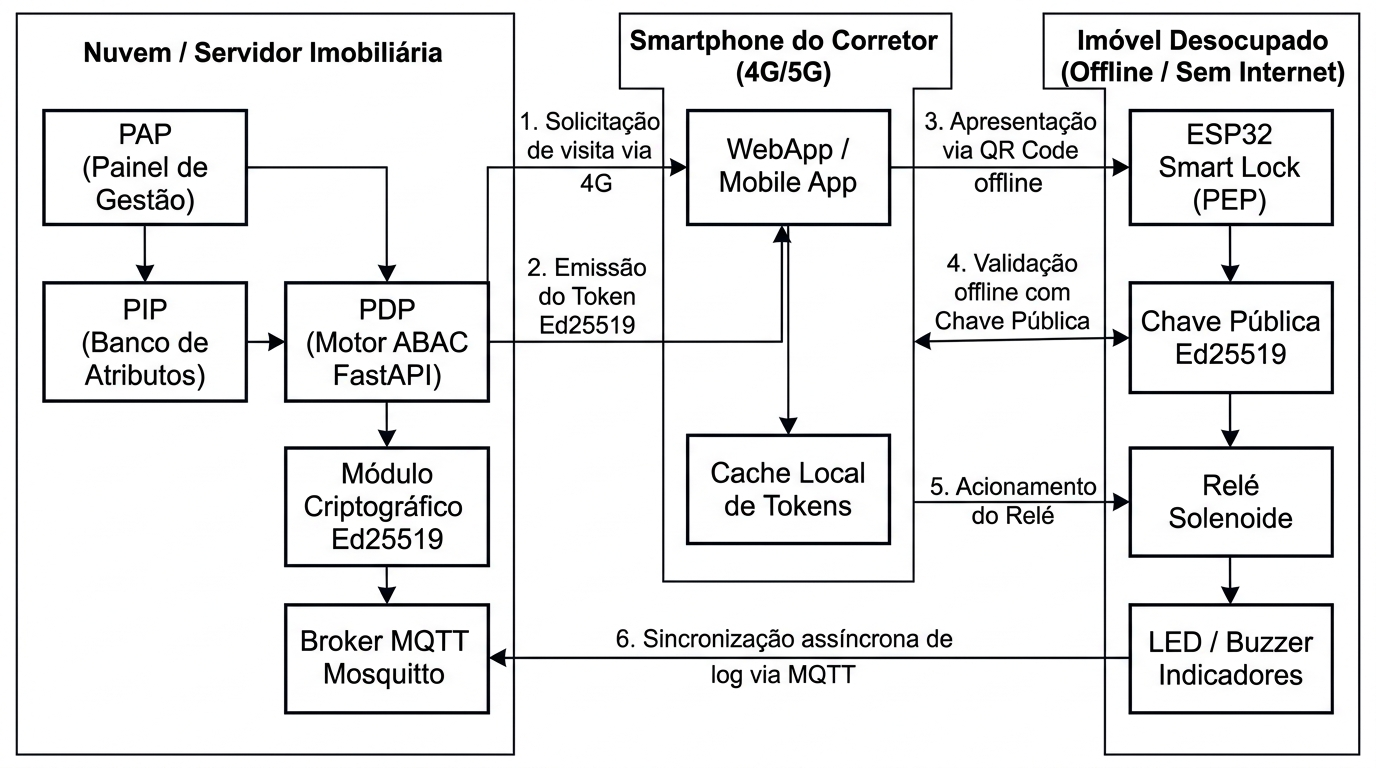
\includegraphics[width=0.92\textwidth]{imagens/01_arquitetura_visao_geral.jpg}
\fonte{Elaborado pelo autor (2026).}
\end{figure}

O ecossistema divide-se em três domínios físicos com responsabilidades bem delimitadas:

\begin{itemize}
    \item \textbf{Nuvem da Imobiliária:} Centraliza os serviços corporativos e a tomada de decisão. Contém o Painel de Gestão (\textit{Policy Administration Point} -- PAP), o repositório de atributos cadastrais (\textit{Policy Information Point} -- PIP), o motor de regras (\textit{Policy Decision Point} -- PDP em FastAPI), o módulo criptográfico detentor da chave privada Ed25519 e o broker MQTT (Eclipse Mosquitto) para recepção das telemetrias de auditoria.
    \item \textbf{Smartphone do Corretor:} Atua como elemento intermediário e portador (\textit{data mule/carrier}) de credenciais e telemetrias. Uma vez que o profissional dispõe de conectividade celular móvel (4G/5G), seu smartphone estabelece a ponte de comunicação entre a nuvem e o imóvel desocupado, requisitando o token pela internet e apresentando-o localmente por leitura óptica.
    \item \textbf{Nó da Fechadura (ESP32):} Atua como Ponto de Aplicação de Políticas (\textit{Policy Enforcement Point} -- PEP) local. Opera em regime estritamente desconectado (\textit{zero local infrastructure}), desprovido de conexão Wi-Fi ou modem celular. Armazena exclusivamente a chave pública da autoridade emissora em memória permanente protegida, garantindo que mesmo o acesso físico ao hardware não exponha segredos capazes de forjar credenciais.
\end{itemize}

O ciclo operacional entre esses domínios executa-se em seis etapas: (1) solicitação de visita via canal celular 4G/5G pelo aplicativo móvel; (2) avaliação de políticas no PDP e assinatura digital do token com a chave privada mestre Ed25519; (3) renderização da credencial em código QR dinâmico na tela do smartphone; (4) verificação determinística da assinatura no microcontrolador ESP32 contra a chave pública gravada no firmware; (5) comutação do relé por 5 segundos para retração do solenoide acompanhada de sinalização visual e sonora; e (6) despacho assíncrono do recibo de confirmação ao broker MQTT via smartphone sob QoS 1 (\textit{at least once}).

% ============================================================
\section{Modelo de Autorização Baseado em Atributos (ABAC)}
\label{sec:modelo-abac}
% ============================================================

\subsection{Transição do RBAC ao ABAC no Contexto Imobiliário}
\label{subsec:rbac-vs-abac}

O modelo de Controle de Acesso Baseado em Papéis (\textit{Role-Based Access Control} -- RBAC) restringe privilégios a partir de funções estáticas atribuídas a usuários. No cenário imobiliário, essa abordagem mostra-se insuficiente: determinar apenas que um indivíduo possui o papel de ``corretor'' não impede que ele ingresse na propriedade fora do horário comercial, acesse unidades vendidas ou entre em imóveis sem agendamento homologado. Tentar contornar essas limitações via RBAC gera explosão de papéis (\textit{role explosion}), tornando a administração impraticável.

O Controle de Acesso Baseado em Atributos (\textit{Attribute-Based Access Control} -- ABAC), adaptado da formulação HABAC$\alpha$ proposta por \citeonline{ameer2022}, soluciona essa restrição avaliando dinamicamente predicados lógicos em tempo de execução:

\begin{equation}
\label{eq:abac-decisao}
\text{Decisão} = f(U_{\text{atrib}},\; D_{\text{atrib}},\; OP_{\text{atrib}},\; ES_{\text{atrib}})
\end{equation}

Em que $U_{\text{atrib}}$ representa os atributos do sujeito solicitante, $D_{\text{atrib}}$ os atributos do dispositivo/imóvel de destino, $OP_{\text{atrib}}$ os parâmetros da ação requerida e $ES_{\text{atrib}}$ as variáveis contextuais do ambiente no instante da avaliação.

\subsection{Dicionário de Atributos do Sistema}
\label{subsec:dicionario-atributos}

O modelo formal implementado organiza treze atributos essenciais para a regulação do acesso às unidades, detalhados no Quadro~\ref{quadro:dicionario-atributos}.

\begin{table}[htbp]
\centering
\footnotesize
\caption{Dicionário de atributos do modelo ABAC projetado.}
\label{quadro:dicionario-atributos}
\begin{tabularx}{\textwidth}{cc p{4.2cm} X}
\toprule
\textbf{Entidade} & \textbf{Símbolo} & \textbf{Atributo} & \textbf{Definição e Tipagem} \\
\midrule
\multirow{4}{*}{Sujeito ($U$)} 
 & $U$ & \texttt{u.id} & String (UUID): Identificador único do corretor. \\
 & $U$ & \texttt{u.role} & Enum: \texttt{CORRETOR\_PARCEIRO}, \texttt{GESTOR}. \\
 & $U$ & \texttt{u.status} & Enum: \texttt{ATIVO}, \texttt{SUSPENSO}, \texttt{PENDENTE}. \\
 & $U$ & \texttt{u.device\_fp} & String (Hash SHA-256): Identificador do smartphone cadastrado. \\
\addlinespace
\multirow{3}{*}{Objeto ($D$)} 
 & $D$ & \texttt{d.lock\_id} & String (Hex): Identificador físico gravado no ESP32. \\
 & $D$ & \texttt{d.status\_imovel} & Enum: \texttt{DISPONIVEL\_VENDA}, \texttt{LOCADO}, \texttt{MANUTENCAO}. \\
 & $D$ & \texttt{d.lock\_state} & Enum: \texttt{TRAVADO}, \texttt{DESTRAVADO}, \texttt{BLOQUEIO}. \\
\addlinespace
\multirow{2}{*}{Ação ($OP$)} 
 & $OP$ & \texttt{op.tipo} & Enum: \texttt{SOLICITAR\_TOKEN}, \texttt{DESTRAVAR\_PORTA}. \\
 & $OP$ & \texttt{op.modo} & Enum: \texttt{OFFLINE\_BEARER}, \texttt{TELEMETRIA}. \\
\addlinespace
\multirow{4}{*}{Ambiente ($ES$)} 
 & $ES$ & \texttt{es.timestamp} & Inteiro (Unix Epoch): Horário de recepção da solicitação. \\
 & $ES$ & \texttt{es.horario\_comercial} & Booleano: \texttt{true} se horário atual estiver entre 08h e 19h. \\
 & $ES$ & \texttt{es.dia\_permitido} & Booleano: Restrição a finais de semana ou feriados. \\
 & $ES$ & \texttt{es.agendamento\_ativo} & Booleano: Confirmação de visita agendada na base imobiliária. \\
\bottomrule
\end{tabularx}
\fonte{Elaborado pelo autor (2026).}
\end{table}

\subsection{Arquitetura Funcional segundo o Padrão NIST SP 800-162}
\label{subsec:arquitetura-nist}

A segregação dos módulos de controle de acesso adota as especificações do padrão NIST SP 800-162, dividindo as responsabilidades de administração, persistência, inferência e aplicação, conforme exposto na Figura~\ref{fig:modelo-abac-nist}.

\begin{figure}[htbp]
\centering
\caption{Arquitetura funcional de controle de acesso ABAC baseada no padrão NIST SP 800-162.}
\label{fig:modelo-abac-nist}
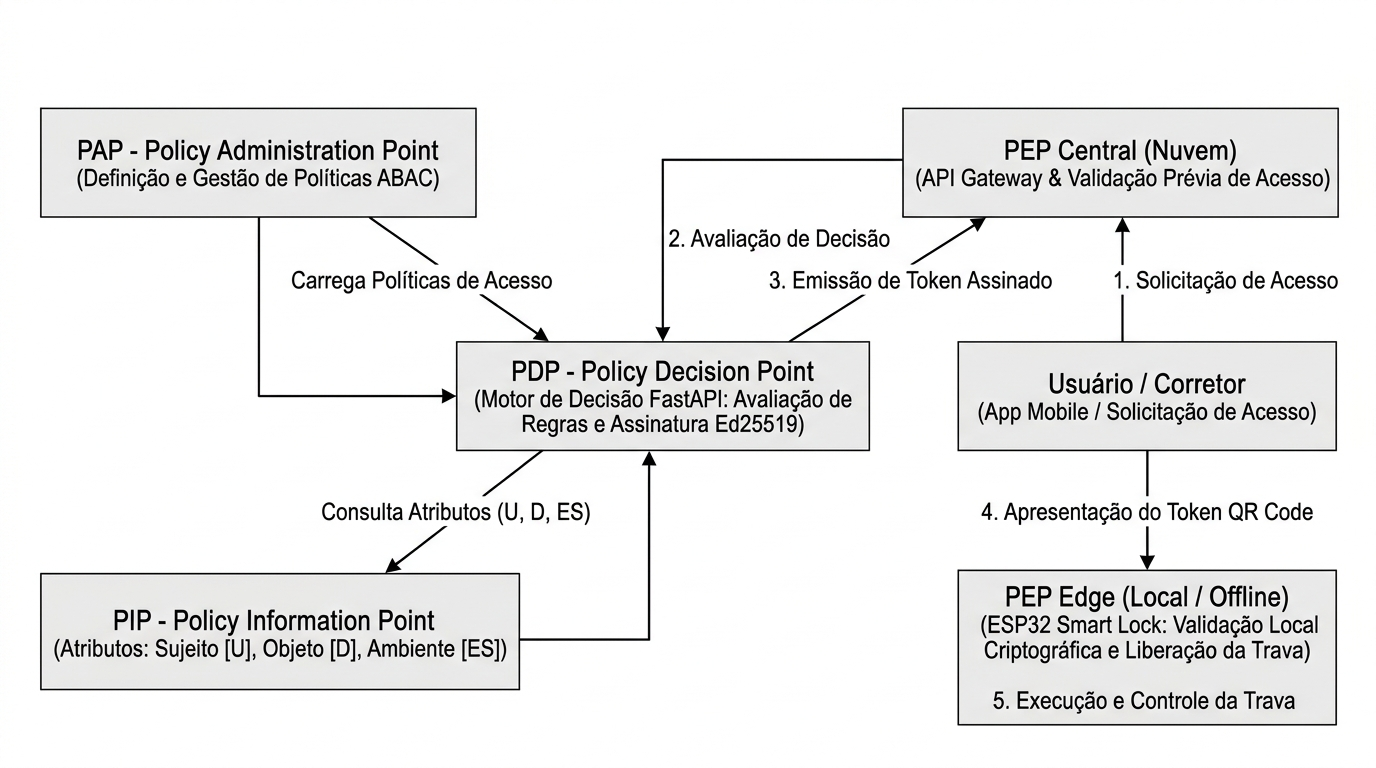
\includegraphics[width=0.78\textwidth, keepaspectratio]{imagens/03_modelo_abac_nist.jpg}
\fonte{Elaborado pelo autor (2026).}
\end{figure}

A interação entre os módulos ocorre de maneira estruturada:
\begin{itemize}
    \item \textbf{PAP (\textit{Policy Administration Point}):} Módulo administrativo em que gestores definem e atualizam as regras de visitação e horários permitidos.
    \item \textbf{PIP (\textit{Policy Information Point}):} Base relacional estruturada que fornece os valores correntes dos atributos vinculados ao usuário, à unidade imobiliária e à agenda.
    \item \textbf{PDP (\textit{Policy Decision Point}):} Motor de inferência construído sobre FastAPI/Python. Processa os dados da requisição, consulta o PIP, confronta as condições estipuladas na política e comanda o módulo criptográfico para emissão do token.
    \item \textbf{PEP Central (\textit{Cloud PEP}):} Ponto de aplicação no API Gateway de nuvem, responsável por barrar requisições malformadas ou com falha de autenticação preliminar.
    \item \textbf{PEP Borda (\textit{Edge PEP}):} Firmware embarcado no ESP32 na porta do imóvel. Recebe a credencial, checa a assinatura digital contra a chave pública e comuta o relé físico.
\end{itemize}

\subsection{Formalização das Regras de Acesso e Algoritmo de Combinação}
\label{subsec:regras-abac}

As políticas de acesso são estruturadas em formato JSON e avaliadas pelo PDP. O Código~\ref{lst:politica-abac} apresenta a regra fundamental aplicada às visitas de corretores parceiros.

\begin{lstlisting}[language=Python, caption={Estrutura da política de autorização ABAC implementada no PDP.}, label={lst:politica-abac}]
{
  "policy_id": "POL_VISITA_IMOVEL_DISPONIVEL",
  "description": "Permite visita de corretores ativos a imoveis disponiveis em horario comercial",
  "target": {
    "action": "SOLICITAR_TOKEN",
    "role": "CORRETOR_PARCEIRO"
  },
  "rules": [
    {
      "rule_id": "REGRA_01_STATUS_CORRETOR",
      "condition": "u.status == 'ATIVO'",
      "effect": "Permit"
    },
    {
      "rule_id": "REGRA_02_STATUS_IMOVEL",
      "condition": "d.status_imovel in ['DISPONIVEL_VENDA', 'DISPONIVEL_LOCACAO']",
      "effect": "Permit"
    },
    {
      "rule_id": "REGRA_03_JANELA_HORARIA",
      "condition": "es.horario_comercial == true and es.dia_permitido == true",
      "effect": "Permit"
    },
    {
      "rule_id": "REGRA_04_VINCULO_AGENDAMENTO",
      "condition": "es.agendamento_ativo == true",
      "effect": "Permit"
    }
  ],
  "rule_combining_algorithm": "deny_overrides"
}
\end{lstlisting}

O mecanismo adota a disciplina de combinação \texttt{deny\_overrides}: caso qualquer uma das regras retorne negação (\textit{Deny}), a requisição é sumariamente recusada pelo servidor, aplicando com rigor o princípio do privilégio mínimo.

% ============================================================
\section{Modelo Criptográfico e Validação Offline}
\label{sec:modelo-criptografico}
% ============================================================

\subsection{O Paradigma da Validação Desconectada (Analogia EMV)}
\label{subsec:analogia-emv}

O nó IoT instalado na porta opera sem conexão à internet no instante em que o corretor se apresenta no local. A concepção adotada baseia-se no princípio empregado pelo padrão bancário internacional EMV (\textit{Europay, Mastercard, Visa}) para transações em terminais desconectados (\textit{offline transaction verification}).

No padrão EMV, o terminal de pagamento não consulta o saldo em conta em tempo real, mas possui gravada a chave pública da autoridade emissora. Ao validar a assinatura digital contida no microprocessador do cartão, o terminal obtém garantia matemática de autenticidade da credencial e integridade dos dados da operação.

No artefato desenvolvido, o PDP na nuvem desempenha o papel de autoridade emissora, detendo a chave privada mestre. O smartphone atua como portador do token assinado. O microcontrolador ESP32 comporta-se de forma análoga ao terminal: a partir da chave pública armazenada em sua memória, autentica o token apresentado localmente sem recorrer a redes externas.

\subsection{Seleção do Algoritmo Criptográfico Ed25519}
\label{subsec:escolha-ed25519}

Microcontroladores de baixo consumo operam sob fortes restrições de memória volátil e capacidade aritmética. Algoritmos assimétricos tradicionais, como RSA-2048, exigem exponenciação modular pesada, demandando elevado tempo de processamento e consumo de memória RAM incompatível com o ESP32.

A criptografia de curvas elípticas contorna essa restrição. O algoritmo selecionado para o projeto foi o Ed25519 (\textit{Edwards-curve Digital Signature Algorithm}), baseado na Curva de Edwards Torcida Curve25519. O Quadro~\ref{quadro:comparativo-cripto} compara as características técnicas de esquemas comuns frente às demandas do nó embarcado.

\begin{table}[htbp]
\centering
\footnotesize
\caption{Comparativo entre esquemas criptográficos para validação em nós IoT embarcados.}
\label{quadro:comparativo-cripto}
\begin{tabularx}{\textwidth}{p{3.2cm} ccc X}
\toprule
\textbf{Critério} & \textbf{RSA-2048} & \textbf{HMAC-SHA256} & \textbf{Ed25519} & \textbf{Impacto no ESP32} \\
\midrule
Tipo de Chave & Assimétrica & Simétrica & Assimétrica & Protege contra cópia física da memória Flash. \\
Tamanho da Chave & 256 bytes & 32 bytes (segredo) & 32 bytes & Reduzida ocupação em memória permanente. \\
Tamanho da Assinatura & 256 bytes & 32 bytes & 64 bytes & Otimizado para pacotes seriais e códigos QR. \\
Tempo de Verificação & 150 a 300 ms & $<$ 1 ms & 1,8 a 3,5 ms & Desempenho quase instantâneo de abertura. \\
Nível de Segurança & 112 bits & 128 bits & 128 bits & Criptograficamente equivalente a RSA de 3072 bits. \\
Ataques de Canal Lateral & Moderada & Boa & Excelente & Imunidade a variações de tempo computacional. \\
\bottomrule
\end{tabularx}
\fonte{Elaborado pelo autor com base em \citeonline{ameer2022} e dados de literatura técnica (2026).}
\end{table}

A adoção do Ed25519 oferece uma vantagem estrutural: como o microcontrolador armazena exclusivamente a chave pública (32 bytes), mesmo que o equipamento seja subtraído fisicamente e sua memória extraída, nenhuma chave privada é comprometida, impedindo a geração forjada de credenciais para outras unidades.

\subsection{Estrutura do Token de Acesso}
\label{subsec:estrutura-token}

O token emitido pelo PDP é compactado em formato serializado JSON. O Código~\ref{lst:payload-token} ilustra a estrutura dos campos transmitidos.

\begin{lstlisting}[language=Python, caption={Estrutura formal do payload do token de acesso emitido pelo PDP.}, label={lst:payload-token}]
{
  "jti": "a7f4b892-91c2-4e88-9d21-f09b578c92a1",
  "sub": "corretor_id_8472",
  "dev": "lock_esp32_imovel_042",
  "nbf": 1774204800,
  "exp": 1774205700,
  "act": "UNLOCK_DOOR",
  "fp":  "e3b0c442...[hash SHA-256 do aparelho]...",
  "sig": "3a8f9c10...[64 bytes assinatura Ed25519]..."
}
\end{lstlisting}

O detalhamento funcional de cada parâmetro constituinte consta no Quadro~\ref{quadro:dicionario-token}.

\begin{table}[htbp]
\centering
\footnotesize
\caption{Dicionário de campos constituintes do token de acesso.}
\label{quadro:dicionario-token}
\begin{tabularx}{\textwidth}{p{1.4cm} p{2.8cm} X}
\toprule
\textbf{Campo} & \textbf{Nome Técnico} & \textbf{Finalidade Funcional} \\
\midrule
\texttt{jti} & JWT ID / Nonce & Identificador universal único (UUIDv4) para prevenção de ataques de repetição. \\
\texttt{sub} & \textit{Subject} & Identificador cadastral do corretor requerente habilitado. \\
\texttt{dev} & \textit{Device Target} & Identificador exclusivo da fechadura destinatária. Evita o uso em portas incorretas. \\
\texttt{nbf} & \textit{Not Before} & Timestamp Unix que estabelece o início da validade da permissão concedida. \\
\texttt{exp} & \textit{Expiration} & Timestamp Unix final de vigência (tempo de vida restrito a 15 minutos). \\
\texttt{act} & \textit{Action} & Ação delegada ao dispositivo físico (\texttt{UNLOCK\_DOOR}). \\
\texttt{fp} & \textit{Device Fingerprint} & Hash vinculado ao aparelho móvel cadastrado \cite{satanasaowapak2021}. \\
\texttt{sig} & \textit{Digital Signature} & Assinatura de 64 bytes gerada pelo PDP com a chave privada mestre Ed25519. \\
\bottomrule
\end{tabularx}
\fonte{Elaborado pelo autor (2026).}
\end{table}

\subsection{Algoritmo de Verificação Local no ESP32}
\label{subsec:algoritmo-verificacao-esp32}

Ao receber o payload serial via interface de leitura, o firmware do ESP32 processa os dados por meio de uma bateria determinística de cinco testes, conforme sumarizado na Figura~\ref{fig:fluxo-validacao-offline}.

\begin{figure}[htbp]
\centering
\caption{Fluxograma de validação determinística de tokens offline no microcontrolador ESP32.}
\label{fig:fluxo-validacao-offline}
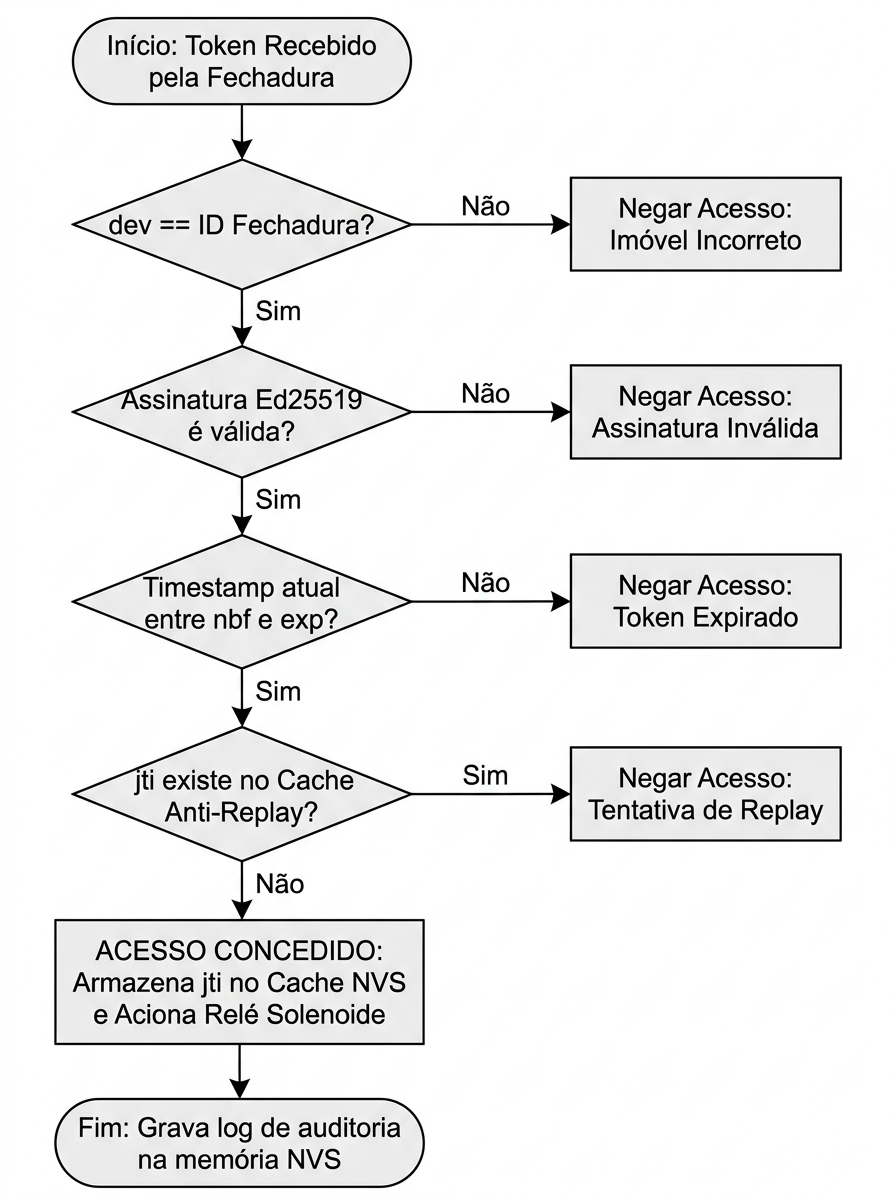
\includegraphics[width=0.88\textwidth]{imagens/02_fluxo_validacao_offline.jpg}
\fonte{Elaborado pelo autor (2026).}
\end{figure}

O fluxo executa-se com término antecipado ao menor indício de inconsistência:
\begin{enumerate}
    \item \textbf{Verificação de Destino (\texttt{dev}):} Compara o campo \texttt{dev} com a identidade física da fechadura gravada na partição de configuração.
    \item \textbf{Verificação Criptográfica (\texttt{sig}):} Invoca a biblioteca \texttt{mbedtls} para recalcular a verificação assimétrica da assinatura com a chave pública mestre.
    \item \textbf{Verificação Temporal (\texttt{nbf} e \texttt{exp}):} Compara o horário interno com a janela permitida.
    \item \textbf{Verificação de Unicidade (\texttt{jti}):} Consulta a partição NVS para checar se o token já foi consumido.
    \item \textbf{Atuação Mecânica:} Persiste o \texttt{jti} no buffer histórico, aciona o relé por 5 segundos e ativa a sinalização audiovisual.
\end{enumerate}

\subsection{Prevenção contra Ataques e Gestão do Buffer Anti-Replay}
\label{subsec:anti-replay}

Para assegurar que interceptações não permitam aberturas indevidas, o sistema projeta as contramedidas estruturadas no Quadro~\ref{quadro:vetores-ataque}.

\begin{table}[htbp]
\centering
\footnotesize
\caption{Matriz de contramedidas de segurança projetadas contra vetores de ataque.}
\label{quadro:vetores-ataque}
\begin{tabularx}{\textwidth}{p{3cm} X p{5.2cm}}
\toprule
\textbf{Vetor de Ataque} & \textbf{Descrição do Ataque} & \textbf{Mecanismo de Defesa do Artefato} \\
\midrule
Replay Attack & Interceptação do código QR para reapresentação posterior ao leitor. & O \texttt{jti} é gravado em buffer circular na memória Flash NVS. Reenvios são barrados. \\
Token Expirado & Uso de credencial legítima após o horário autorizado. & Confronto do timestamp \texttt{exp} com descarte de tokens com TTL estourado. \\
Adulteração de Payload & Tentativa de forjar horário de término ou trocar identificador de imóvel. & A assinatura Ed25519 é invalidada matematicamente; leitura é recusada. \\
Imóvel Incorreto & Uso de token da Unidade A na Unidade B. & O identificador \texttt{dev} diverge da identidade estática da fechadura. \\
Compartilhamento & Envio de captura de tela para terceiro não credenciado. & O hash \texttt{fp} vincula o token ao smartphone registrado \cite{satanasaowapak2021}. \\
Subtração do Nó & Furto físico do dispositivo para clonagem de chaves. & O microcontrolador guarda apenas a chave pública; chaves privadas ficam isoladas na nuvem. \\
\bottomrule
\end{tabularx}
\fonte{Elaborado pelo autor (2026).}
\end{table}

A gestão do buffer anti-replay dimensiona uma fila circular na memória flash NVS com capacidade para reter até 200 identificadores \texttt{jti}. Com validade restrita a 15 minutos (900 segundos) por token, o buffer de 200 posições atende com margem à rotina de visitas, ocupando menos de 8~KB na partição de dados.

% ============================================================
\section{Fluxo de Operação de Ponta a Ponta}
\label{sec:fluxo-ponta-a-ponta}
% ============================================================

A operação do ecossistema divide-se em três etapas coordenadas: emissão online do token pela nuvem, validação local offline no imóvel e sincronização assíncrona de auditoria. A Figura~\ref{fig:diagrama-sequencia-visita} expõe o diagrama de sequência detalhado.

\begin{figure}[htbp]
\centering
\caption{Diagrama de sequência ponta a ponta do processo de requisição, validação e auditoria de visitas.}
\label{fig:diagrama-sequencia-visita}
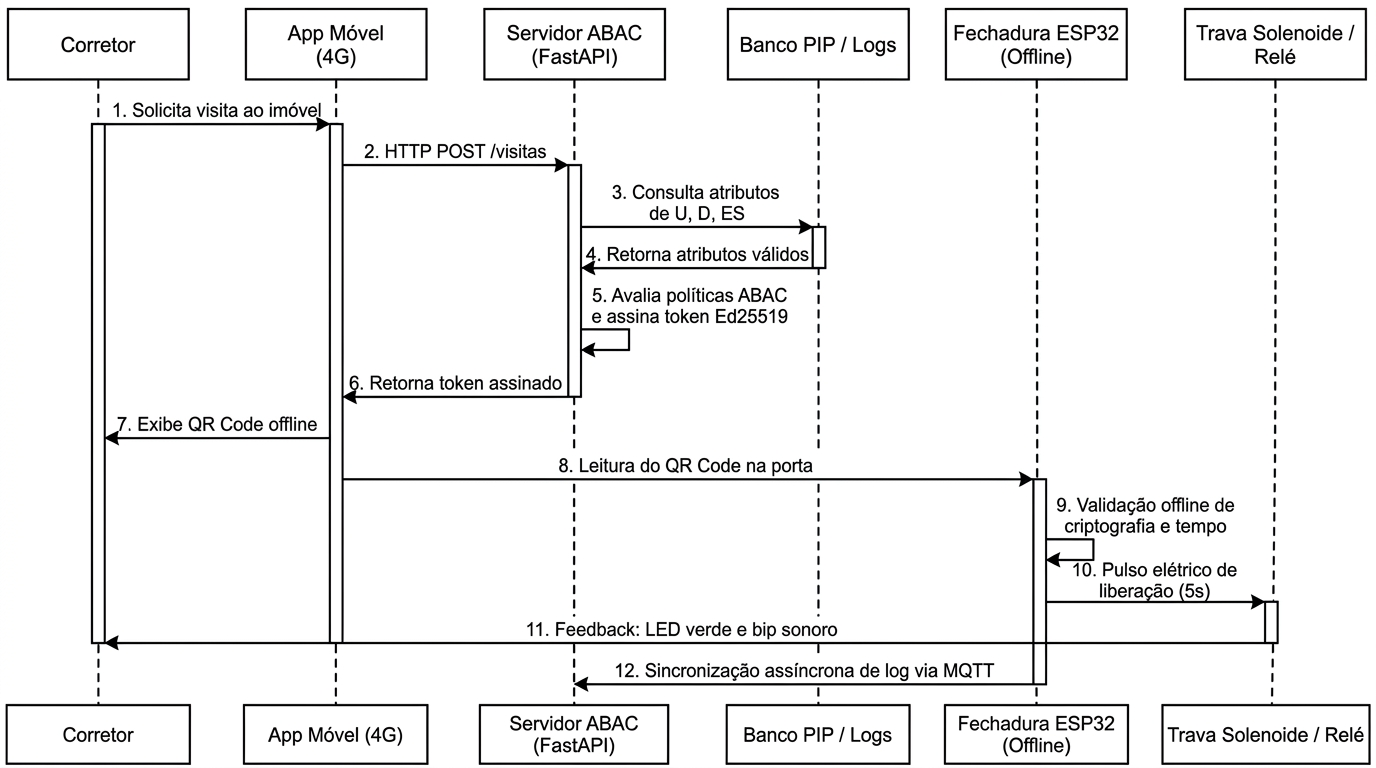
\includegraphics[width=0.95\textwidth]{imagens/04_diagrama_sequencia_visita.jpg}
\fonte{Elaborado pelo autor (2026).}
\end{figure}

\subsection{Fase 1: Solicitação e Emissão do Token (Online)}
\label{subsec:fluxo-fase-emissao}

\begin{enumerate}
    \item Ao se aproximar do imóvel, o corretor aciona o aplicativo em seu smartphone conectado à rede celular (4G/5G).
    \item O aplicativo envia uma requisição HTTP via TLS pelo endpoint \path{/api/v1/access/request-token} ao servidor central, informando suas credenciais, identificador do imóvel e assinatura digital do aparelho móvel.
    \item O PDP recebe a requisição e interroga o banco relacional (PIP) para obter a situação cadastral do corretor, regras do condomínio e agendamento ativo.
    \item O motor ABAC processa as condições declaradas na política ativa.
    \item Havendo conformidade, o módulo criptográfico gera o payload com identificador \texttt{jti} inédito, calcula a assinatura digital com a chave privada mestre Ed25519 e devolve o pacote codificado em JSON sob código HTTP 200. Havendo inconformidade, o servidor devolve código HTTP 403 com a justificativa de negação.
    \item O aplicativo retém a credencial em cache seguro e gera na tela um código QR dinâmico com o payload serializado.
\end{enumerate}

\subsection{Fase 2: Apresentação e Validação Local (Offline)}
\label{subsec:fluxo-fase-validacao}

\begin{enumerate}
    \item O corretor aproxima a tela do smartphone da interface de leitura associada ao microcontrolador ESP32 na porta do imóvel.
    \item O microcontrolador processa a cadeia de caracteres recebida e reconstrói o payload em memória de trabalho.
    \item O firmware executa a rotina de validação: confere o código \texttt{dev}, verifica a assinatura Ed25519 com a chave pública instalada, atesta a janela de vigência (\texttt{nbf} e \texttt{exp}) e busca o \texttt{jti} no buffer anti-replay.
    \item Comprovada a autenticidade e tempestividade do token, o pino GPIO 23 é levado a nível lógico alto, excitando a bobina do relé por 5 segundos para retração do pino solenoide. Concomitantemente, o LED verde (GPIO 2) acende e o \textit{buzzer} (GPIO 18) emite um sinal agudo.
    \item O identificador \texttt{jti} é gravado na memória Flash NVS local.
\end{enumerate}

\subsection{Fase 3: Sincronização Assíncrona e Auditoria}
\label{subsec:fluxo-fase-auditoria}

\begin{enumerate}
    \item Concluída a abertura física, o aplicativo do corretor gera um recibo assinado contendo o \texttt{jti} consumido e o timestamp da operação.
    \item O smartphone despacha o recibo ao broker MQTT corporativo (Eclipse Mosquitto) no canal \texttt{imobiliaria/auditoria/acessos}, via conexão celular e nível de serviço QoS 1 (\textit{at least once}).
    \item O serviço de auditoria em nuvem armazena a mensagem na base relacional da imobiliária, garantindo rastreabilidade sem violar o isolamento do nó físico.
\end{enumerate}

% ============================================================
\section{Stack Tecnológica e Especificação do Firmware}
\label{sec:stack-tecnologica}
% ============================================================

\subsection{Mapeamento dos Componentes Tecnológicos}
\label{subsec:mapeamento-stack}

A escolha das ferramentas orientou-se pela padronização acadêmica e viabilidade de execução em sistemas embarcados restritos. O Quadro~\ref{quadro:stack-tecnologica} sintetiza os componentes da solução.

\begin{table}[htbp]
\centering
\footnotesize
\caption{Mapeamento da pilha tecnológica empregada no desenvolvimento do artefato.}
\label{quadro:stack-tecnologica}
\begin{tabularx}{\textwidth}{p{2.8cm} p{4.2cm} X}
\toprule
\textbf{Camada / Módulo} & \textbf{Tecnologia Selecionada} & \textbf{Justificativa Técnica e Acadêmica} \\
\midrule
Nó da Fechadura (PEP) & ESP32 DevKit v1 (Xtensa LX6 Dual-Core 240 MHz) & Plataforma consolidada na literatura de automação e segurança IoT residencial \cite{vardakis2024}. \\
Linguagem do Firmware & C/C++ sobre PlatformIO / Framework Arduino & Controle determinístico de memória e integração nativa à biblioteca criptográfica \texttt{mbedtls}. \\
Servidor de Políticas (PDP) & Python 3.11+ com FastAPI & Arquitetura assíncrona ASGI de alto rendimento, tipagem estrita com Pydantic e documentação OpenAPI. \\
Biblioteca Criptográfica & PyNaCl (Servidor) e mbedtls (ESP32) & Implementações de referência do algoritmo Ed25519 resistentes a vazamento por canal lateral. \\
Broker de Mensageria & Eclipse Mosquitto v2.0+ & Padrão aberto com suporte nativo a MQTT v3.1.1/v5.0, baixo consumo de memória ($<$ 10~MB) e garantia QoS 1. \\
Ambiente de Simulação & Wokwi IoT Simulator & Plataforma com emulação precisa de registradores do ESP32, suporte a rede virtual e periféricos. \\
Interface do Corretor & Progressive Web App (PWA) em HTML5/JS & Permite acesso multiplataforma via navegador móvel sem fricção de distribuição em lojas de aplicativos. \\
Ferramentas de Carga & Locust e Pytest & Automação de testes de estresse, injeção de requisições concorrentes e mensuração de latências. \\
\bottomrule
\end{tabularx}
\fonte{Elaborado pelo autor (2026).}
\end{table}

\subsection{Organização Modular do Firmware no ESP32}
\label{subsec:modulos-firmware}

O software a ser embarcado no microcontrolador organiza-se em três módulos desacoplados:

\begin{description}
    \item[\texttt{crypto\_verifier.cpp}:] Isola o subsistema criptográfico. Contém a chave pública mestre de 32 bytes (\texttt{SERVER\_PUBLIC\_KEY}) gravada em memória de programa (\texttt{PROGMEM}). Inicializa as estruturas da biblioteca \texttt{mbedtls} e disponibiliza a função \texttt{verify\_ed25519\_signature(payload, signature, pubkey)}.
    \item[\texttt{token\_validator.cpp}:] Executa a análise semântica dos dados recebidos. Utiliza a biblioteca \texttt{ArduinoJson} com alocação estática de memória (\texttt{StaticJsonDocument}) para prevenir fragmentação de heap. Realiza o confronto do campo \texttt{dev}, checagem de janelas temporais e iteração sobre a lista anti-replay mantida na NVS.
    \item[\texttt{lock\_actuator.cpp}:] Gerencia a interface com atuadores e sinalizadores físicos. Controla os estados dos pinos GPIO por temporizadores não bloqueantes baseados na função \texttt{millis()}, eliminando bloqueios de processamento.
\end{description}

\subsection{Endpoints e Motor de Inferência em FastAPI}
\label{subsec:endpoints-api}

O backend construído sobre FastAPI disponibiliza três pontos de entrada principais:

\begin{itemize}
    \item \texttt{POST /api/v1/access/request-token}: Endpoint principal de requisição. Recebe as credenciais do corretor, ID do imóvel e dados contextuais. Aciona a função de inferência ABAC, consulta a base relacional e, havendo decisão afirmativa, emprega o método \texttt{crypto\_sign\_detached} da biblioteca \texttt{PyNaCl} para produzir a assinatura do token.
    \item \texttt{PATCH /api/v1/corretores/\{id\}/status}: Ponto de gestão cadastral utilizado por administradores. Permite alterar o status de um corretor de \texttt{ATIVO} para \texttt{SUSPENSO}. Modificações refletem-se instantaneamente no banco relacional, bloqueando emissões subsequentes de tokens.
    \item \texttt{GET /api/v1/imoveis/\{id\}/logs}: Consulta a série histórica de acessos registrados para uma determinada unidade imobiliária, viabilizando relatórios gerenciais de auditoria.
\end{itemize}

\subsection{Estrutura de Mensageria e Tópicos MQTT}
\label{subsec:topicos-mqtt}

Para garantir a rastreabilidade dos eventos, as mensagens transitam pelo broker Eclipse Mosquitto estruturadas sob uma hierarquia padronizada de tópicos:

\begin{lstlisting}[language=bash, caption={Estrutura hierárquica de tópicos MQTT empregada no sistema.}, label={lst:topicos-mqtt}]
imobiliaria/
+-- imoveis/{imovel_id}/
|   +-- status          # Telemetria: Online/Offline/Bateria
|   +-- revogacoes      # Broadcast de revogacao emergencial
|   +-- telemetria      # Tempo de resposta e diagnosticos
+-- auditoria/
|   +-- acessos         # Recibos de acessos executados
|   +-- alertas         # Tentativas com token invalido
+-- comandos/{imovel_id}/
    +-- emergencia      # Bloqueio forcado administrativo
\end{lstlisting}

O pacote de auditoria remetido ao canal \texttt{imobiliaria/auditoria/acessos} adota a estrutura esquemática apresentada no Código~\ref{lst:pacote-auditoria}.

\begin{lstlisting}[language=Python, caption={Formato esquemático do pacote de auditoria despachado via MQTT QoS 1.}, label={lst:pacote-auditoria}]
{
  "event_id": "evt_998124_ack",
  "timestamp": 1774204850,
  "imovel_id": "lock_esp32_imovel_042",
  "corretor_id": "corretor_id_8472",
  "jti_utilizado": "a7f4b892-91c2-4e88-9d21-f09b578c92a1",
  "resultado": "ACESSO_CONCEDIDO",
  "latencia_validacao_ms": 2.45,
  "latencia_comunicacao_ms": 178.30
}
\end{lstlisting}

% ============================================================
\section{Bancada de Simulação Virtual no Wokwi}
\label{sec:bancada-simulacao}
% ============================================================

\subsection{Mapeamento do Circuito Eletrônico e Pinout}
\label{subsec:circuito-wokwi}

O circuito virtual foi modelado no Wokwi Simulator utilizando o módulo virtual ESP32 DevKit v1. As ligações elétricas aos periféricos virtuais utilizam o mapa de pinos indicado no Quadro~\ref{quadro:pinout-esp32}.

\begin{table}[htbp]
\centering
\footnotesize
\caption{Mapeamento dos pinos GPIO e periféricos no circuito virtual ESP32.}
\label{quadro:pinout-esp32}
\begin{tabularx}{\textwidth}{c c p{3.8cm} X}
\toprule
\textbf{Pino GPIO} & \textbf{Direção} & \textbf{Dispositivo Conectado} & \textbf{Comportamento e Função} \\
\midrule
GPIO 23 & Saída (Digital) & Módulo Relé Solenoide & Nível ALTO comuta o relé por 5 segundos para liberar a trava. \\
GPIO 2 & Saída (Digital) & LED Verde & Pulso luminoso que indica validação e liberação do acesso. \\
GPIO 4 & Saída (Digital) & LED Vermelho & Sinaliza rejeição (token inválido, expirado ou unidade divergente). \\
GPIO 18 & Saída (PWM) & Buzzer Piezoelétrico & Emite um tom agudo para sucesso e dois graves para rejeição. \\
GPIO 16 / 17 & Entrada/Saída & Porta Serial / Leitor RX/TX & Recepção dos dados brutos correspondentes à leitura do código. \\
\bottomrule
\end{tabularx}
\fonte{Elaborado pelo autor (2026).}
\end{table}

A topologia das conexões entre pinos, componentes e referências de terra (GND) é parametrizada no arquivo descritivo \texttt{diagram.json}, reproduzido no Código~\ref{lst:diagram-wokwi}.

\begin{lstlisting}[language=Python, caption={Arquivo descritivo diagram.json do circuito virtual no simulador Wokwi.}, label={lst:diagram-wokwi}]
{
  "version": 1,
  "author": "Controle de Acesso IoT - TCC",
  "editor": "wokwi",
  "parts": [
    { "type": "wokwi-esp32-devkit-v1", "id": "esp", "top": 0, "left": 0, "attrs": {} },
    { "type": "wokwi-relay-module", "id": "relay", "top": 100, "left": 150, "attrs": {} },
    { "type": "wokwi-led", "id": "led_green", "top": -50, "left": 120, "attrs": { "color": "green" } },
    { "type": "wokwi-led", "id": "led_red", "top": -50, "left": 160, "attrs": { "color": "red" } },
    { "type": "wokwi-buzzer", "id": "buzzer", "top": -50, "left": 200, "attrs": {} }
  ],
  "connections": [
    [ "esp:TX", "relay:IN", "green", [ "h20", "v40" ] ],
    [ "esp:D2", "led_green:A", "green", [ "h10", "v-30" ] ],
    [ "esp:D4", "led_red:A", "red", [ "h10", "v-30" ] ],
    [ "esp:D18", "buzzer:2", "blue", [ "h10", "v-30" ] ],
    [ "esp:GND.1", "relay:GND", "black", [ "h0" ] ],
    [ "esp:GND.1", "led_green:C", "black", [ "h0" ] ],
    [ "esp:GND.1", "led_red:C", "black", [ "h0" ] ],
    [ "esp:GND.1", "buzzer:1", "black", [ "h0" ] ]
  ]
}
\end{lstlisting}

% ============================================================
\section{Comportamentos Esperados nos Cenários de Demonstração}
\label{sec:resultados-demonstracao}
% ============================================================

Em alinhamento com a etapa de demonstração da DSR e os objetivos específicos do projeto, estruturam-se os comportamentos projetados para os três cenários operacionais que serão submetidos a ensaios em bancada virtual.

\subsection{Cenário 1: Comportamento Esperado no Fluxo Nominal}
\label{subsec:res-cenario-1}

No fluxo nominal, prevê-se que o corretor com cadastro ativo requisite a entrada para um imóvel disponível dentro do horário comercial e com agendamento homologado.

Espera-se que o motor ABAC (PDP) execute a inferência lógica em tempo reduzido ($< 50$~ms) e invoque o módulo criptográfico para assinatura Ed25519 ($< 5$~ms). Ao apresentar o código QR renderizado na tela do celular à interface óptica do ESP32 na bancada simulada, o comportamento projetado consiste em:
\begin{enumerate}
    \item Conclusão da verificação matemática da assinatura digital em menos de 10~ms;
    \item Comutação do pino GPIO 23 para nível lógico alto por exatamente 5 segundos, acionando a bobina do relé solenoide;
    \item Acendimento do LED verde de confirmação e emissão de pulso agudo no buzzer;
    \item Transmissão assíncrona bem-sucedida do recibo de confirmação pelo aplicativo celular ao broker MQTT, sem perda de pacotes sob QoS 1.
\end{enumerate}

\subsection{Cenário 2: Comportamento Esperado frente a Acessos Inválidos e Ataques}
\label{subsec:res-cenario-2}

Para os ensaios negativos previstos (CT-2.1 a CT-2.4), a hipótese central de segurança requer uma taxa de contenção de 100\% de bloqueio efetivo na extremidade desconectada, sem qualquer falso positivo de concessão:

\begin{itemize}
    \item \textbf{CT-2.1 (Token Expirado):} Diante de tokens com timestamp posterior ao campo \texttt{exp}, espera-se que o firmware efetue o descarte imediato por estouro de TTL, acionando o LED vermelho (GPIO 4) e registrando a tentativa no log local sem comutação do relé.
    \item \textbf{CT-2.2 (Imóvel Divergente):} Caso um token emitido para a Unidade A seja apresentado na fechadura da Unidade B, espera-se que a checagem do campo \texttt{dev} falhe no primeiro estágio algorítmico, bloqueando o processamento antes mesmo da computação criptográfica.
    \item \textbf{CT-2.3 (Assinatura Forjada por Adulteração de Payload):} Diante de adulterações intencionais de bits em campos como vigência ou identificador de usuário, espera-se que a função \texttt{verify\_ed25519} retorne falso deterministicamente, impedindo a liberação física da porta.
    \item \textbf{CT-2.4 (Ataque de Repetição / \textit{Replay}):} Caso uma credencial consumida anteriormente seja apresentada de forma reincidente, espera-se que a rotina de busca na tabela circular NVS identifique a presença do identificador \texttt{jti}, barrando o acesso por duplicidade.
\end{itemize}

\subsection{Cenário 3: Comportamento Esperado na Revogação Cadastral}
\label{subsec:res-cenario-3}

Para a hipótese de revogação cadastral de um corretor na imobiliária, o comportamento projetado divide-se em duas respostas coordenadas:

No ambiente em nuvem, projeta-se que a alteração do status para \texttt{SUSPENSO} reflita de forma imediata no banco relacional (PIP). Requisições subsequentes submetidas pelo aplicativo devem ser indeferidas pelo PDP com código HTTP 403 (\textit{Forbidden}), impedindo a emissão de novos tokens.

No nó da fechadura desconectado, o controle do risco residual decorrente de credenciais geradas instantes antes da suspensão deve ser contido pela expiração temporal intrínseca: o token permanecerá operável apenas durante o intervalo remanescente de seu tempo de vida (TTL máximo de 15 minutos). Esgotada essa janela, o relógio interno do microcontrolador rejeitará o token por expiração, ao passo que tentativas de reuso dentro da janela serão inviabilizadas pelo mecanismo anti-replay.

% ============================================================
\section{Resultados Esperados e Discussão de Hipóteses}
\label{sec:analise-quantitativa}
% ============================================================

Em consonância com o protocolo experimental planejado na metodologia, estabelecem-se as metas de desempenho e as hipóteses analíticas que balizarão a coleta de dados durante os ensaios práticos.

\subsection{Hipóteses de Desempenho Temporal e Latência}
\label{subsec:res-desempenho-temporal}

A avaliação temporal contempla quatro métricas em cadeia: o tempo de decisão das políticas ABAC (M1), o tempo de cálculo da assinatura assimétrica Ed25519 no servidor (M2), o tempo de verificação matemática da assinatura no microcontrolador ESP32 (M3) e o tempo total de resposta perceptível pelo usuário (M4).

Para a inferência ABAC (M1), a meta de tempo médio inferior a 50~ms apoia-se em estudos prévios de motores de políticas contextuais. \citeonline{ameer2022} observaram tempos de decisão entre 15 e 40~ms para regras HABAC em servidores de aplicação. Como a implementação utiliza o framework assíncrono FastAPI (ASGI) associado a consultas indexadas no banco relacional (PIP), o limite de 50~ms garante que a avaliação das políticas lógicas sob a disciplina \texttt{deny\_overrides} ocorra sem bloqueio de threads de I/O.

Para a assinatura digital no servidor (M2), a meta de tempo inferior a 5~ms decorre das características computacionais da Curva de Edwards. Utilizando a biblioteca \texttt{PyNaCl} (baseada na implementação de referência \texttt{libsodium} em C), operações com o algoritmo Ed25519 em processadores de servidor x86-64 consomem tipicamente entre 0,05 e 1,5~ms \cite{hanblockchainoffline2018}. A margem de 5~ms absorve variações sob concorrência de requisições sem degradar a capacidade de resposta do backend.

Na extremidade desconectada, a verificação da assinatura Ed25519 no microcontrolador ESP32 a 240~MHz (M3) tem como meta estrita um tempo inferior a 10~ms. Essa delimitação ganha relevância quando confrontada com esquemas criptográficos tradicionais: \citeonline{hanotmpp2l2020} mediram uma latência de 339~ms para verificação assimétrica baseada em RSA-2048 em um microprocessador ARM Cortex-A7, atraso já perceptível ao usuário. No ESP32, a multiplicação de ponto na curva Curve25519 via biblioteca \texttt{mbedtls} consome menos de 800.000 ciclos de clock (cerca de 2 a 3,5~ms a 240~MHz). O teto de 10~ms fornece margem segura para trocas de contexto no FreeRTOS, garantindo que o destravamento ocorra de forma quase instantânea na porta.

Para a latência total ponta a ponta (M4) --- englobando tráfego de rede celular 4G/5G (150 a 250~ms), inferência em nuvem M1+M2 ($<$ 55~ms), leitura óptica do QR Code e verificação local M3 ($<$ 10~ms) ---, a meta fixada é inferior a 500~ms. Esse patamar apoia-se em diretrizes clássicas de ergonomia computacional (limite de 1 segundo para manutenção do fluxo contínuo de pensamento sem percepção de lentidão) e nas conclusões de \citeonline{satanasaowapak2021} sobre o tempo aceitável em fechaduras inteligentes residenciais.

\subsection{Restrições e Consumo de Recursos Computacionais no ESP32}
\label{subsec:res-consumo-recursos}

Em nós embarcados que operam de forma isolada, a gestão de memória determina a estabilidade operacional contínua. A métrica M5 estabelece que o consumo de memória RAM Heap no ESP32 não ultrapasse 120~KB durante o pico de decodificação JSON e verificação criptográfica. Fisicamente, o ESP32 dispõe de 520~KB de SRAM interna, dos quais aproximadamente 280 a 300~KB permanecem utilizáveis pela aplicação após a carga do FreeRTOS e pilhas nativas. O teto de 120~KB assegura que o firmware ocupe menos de 40\% da memória dinâmica disponível, mantendo margem livre contínua superior a 150~KB. Essa folga, associada à alocação estática com a biblioteca \texttt{ArduinoJson} (\texttt{StaticJsonDocument}), previne fragmentação de heap e falhas por estouro de memória (\textit{Out-Of-Memory}) \cite{vardakis2024}.

Para a memória permanente Flash ROM (M6), a meta restringe a ocupação do binário a menos de 35\% da partição de aplicação. O ESP32 DevKit v1 padrão integra 4~MB (4.096~KB) de memória Flash SPI. Em arquiteturas embarcadas de produção, adota-se o esquema de particionamento duplo para atualizações remotas seguras (\textit{Over-The-Air} -- OTA), no qual existem duas partições de aplicação espelhadas (\texttt{app0} e \texttt{app1}) com cerca de 1.300 a 1.400~KB cada (~32\% a 35\% da flash total). Manter o binário estático abaixo de 35\% é um requisito técnico mandatório para assegurar a viabilidade de atualização e mecanismos de recuperação automática (\textit{rollback}) \cite{simperf2024}.

\subsection{Capacidade de Mensageria e Eficácia de Segurança Projetada}
\label{subsec:res-vazao-seguranca}

Para a métrica M7, a meta de suportar mais de 100 mensagens por segundo no broker Eclipse Mosquitto decorre do dimensionamento de pico de administradoras imobiliárias de médio e grande porte. Mesmo em carteiras com centenas de propriedades e dezenas de corretores ativos em campo nos horários de maior visitação (início da tarde e finais de semana), a taxa de check-ins concorrentes raramente atinge dezenas de acessos por segundo. Como o broker Mosquitto foi desenvolvido em linguagem C com arquitetura assíncrona leve \cite{shauto2024}, a meta de 100 msg/s sob entrega garantida QoS 1 assegura uma margem de folga de cinco a dez vezes sobre o tráfego estimado, sem risco de enfileiramento ou descarte de pacotes de auditoria \cite{ameer2022}.

Por fim, a métrica M8 exige 100\% de bloqueio efetivo frente a tentativas anômalas (CT-2.1 a CT-2.4). Em controle de acesso físico a propriedades desocupadas, a tolerância a falsos positivos de concessão é zero. A fundamentação é matemática: a verificação de assinatura digital sobre curvas de Edwards é uma operação determinística estrita; qualquer alteração de um único bit no payload serializado invalida a prova criptográfica, forçando o algoritmo a retornar falso. Aliado ao buffer circular na partição NVS que impede a reutilização de identificadores \texttt{jti}, o sistema garante a rejeição categórica de acessos expirados, adulterados ou duplicados \cite{satanasaowapak2021}.

\subsection{Quadro Consolidado de Metas e Resultados Esperados}
\label{subsec:quadro-consolidado-resultados}

O Quadro~\ref{quadro:resultados-experimentais} consolida as variáveis de avaliação, as metas numéricas projetadas, os critérios de tolerância e a fundamentação teórica de cada parâmetro a ser aferido nas baterias de 50 repetições.

\begin{table}[htbp]
\centering
\footnotesize
\caption{Quadro consolidado de metas quantitativas e resultados esperados da avaliação experimental.}
\label{quadro:resultados-experimentais}
\begin{tabularx}{\textwidth}{c p{3.6cm} c p{3.2cm} X}
\toprule
\textbf{\#} & \textbf{Variável / Métrica} & \textbf{Meta} & \textbf{Critério de Aceitação} & \textbf{Fundamentação Teórica na Literatura} \\
\midrule
M1 & Latência Decisão ABAC (ms) & $<$ 50 & Ausência de bloqueios de thread no servidor. & Arquitetura assíncrona ASGI/FastAPI com regras JSON compiladas \cite{ameer2022}. \\
\addlinespace
M2 & Assinatura Ed25519 (ms) & $<$ 5 & Execução em tempo constante sem canal lateral. & Operação algébrica otimizada da biblioteca PyNaCl/libsodium \cite{hanblockchainoffline2018}. \\
\addlinespace
M3 & Verificação no ESP32 (ms) & $<$ 10 & Operação matemática instantânea no microcontrolador. & Desempenho de curvas elípticas Curve25519 a 240~MHz via \texttt{mbedtls} \cite{simperf2024}. \\
\addlinespace
M4 & Latência Ponta a Ponta (ms) & $<$ 500 & Tempo total imperceptível ao usuário na porta. & Limites de usabilidade e tolerância humana em IoT \cite{satanasaowapak2021}. \\
\addlinespace
M5 & Memória RAM Heap (KB) & $<$ 120 & Folga contínua $>$ 150~KB sem vazamento de memória. & Alocação estática com ArduinoJson para evitar fragmentação de heap \cite{vardakis2024}. \\
\addlinespace
M6 & Ocupação Flash ROM (\%) & $<$ 35 & Binário compacto em partição de 4~MB. & Eficiência de código em C/C++ embarcado sobre FreeRTOS \cite{simperf2024}. \\
\addlinespace
M7 & Vazão MQTT (msg/s) & $>$ 100 & Zero descarte de pacotes sob nível QoS 1. & Protocolo MQTT leve para telemetria em brokers assíncronos \cite{ameer2022,shauto2024}. \\
\addlinespace
M8 & Taxa Bloqueio Ataques (\%) & 100 & Índice zero de falsos positivos de concessão. & Robustez matemática da assinatura Ed25519 e buffer anti-replay NVS \cite{satanasaowapak2021}. \\
\bottomrule
\end{tabularx}
\fonte{Elaborado pelo autor com base nas diretrizes de projeto e na literatura (2026).}
\end{table}

\subsection{Discussão Teórica e Confronto de Hipóteses com o Estado da Arte}
\label{subsec:discussao-comparativa}

A estruturação das metas do artefato estabelece vantagens teóricas frente aos trabalhos correlatos mapeados na literatura.

Em comparação com o protótipo de \citeonline{hanotmpp2l2020}, que reportou latência de verificação assimétrica de 339~ms em um microprocessador ARM Cortex-A7 utilizando chaves RSA, a meta projetada neste trabalho (M3 $<$ 10~ms com o algoritmo Ed25519) representa uma redução de magnitude superior a trinta vezes no tempo de cálculo no ESP32. Esse avanço decorre da eficiência aritmética das curvas elípticas de Edwards frente às exponenciações modulares pesadas exigidas pelo padrão RSA tradicional.

Frente ao trabalho de \citeonline{satanasaowapak2021}, cuja fechadura baseada em QR Code e senhas temporárias (OTP) depende de enlace local Wi-Fi para recepção de comandos na residência, a proposta aqui apresentada elimina completamente a dependência de infraestrutura de rede no imóvel. O transporte da credencial ocorre por leitura óptica unidirecional e a auditoria é transferida assincronamente à rede celular do próprio smartphone do corretor, eliminando a exposição de portas de rede da fechadura a ataques cibernéticos locais.

Por sua vez, em relação ao modelo HABAC$\alpha$ formalizado por \citeonline{ameer2022}, projetado para residências dotadas de conectividade permanente e gateways de borda ativos, o presente trabalho adapta o paradigma de autorização contextual para o cenário de vacância imobiliária. A inteligência decisória permanece na nuvem corporativa da imobiliária, enquanto o nó físico no imóvel restringe-se a validar a prova criptográfica assinada e a aplicar restrições temporais estritas.

A confirmação dessas hipóteses de desempenho durante a fase de testes empíricos do trabalho permitirá validar a viabilidade de fechaduras inteligentes baseadas em IoT operando com segurança e rastreabilidade plena em ambientes desprovidos de conexão de rede local.

% !TeX root = main.tex
\chapter{Conclusão}
\label{cap:conclusao}
Apresente:

- resumo dos resultados
- contribuição da pesquisa
- limitações
- sugestões para trabalhos futuros

\section{Trabalhos futuros}

% ----------------------------------------------------------

\postextual

% ----------------------------------------------------------
% Referências bibliográficas
% ----------------------------------------------------------
%\bibliography{bibliografia}
\bibliography{referencias}
% ----------------------------------------------------------

%---------------------------------------------------------------------
% INDICE REMISSIVO (descomente caso utilize \makeindex e \index)
%---------------------------------------------------------------------
%\phantompart
%\printindex
%---------------------------------------------------------------------

\end{document}